% Define all the needed variable like it is shown in the var.tex.example 
% (Just copy the var.tex.example file and remove the ".example" from the filename.)
% specify the relative path from the main file to the folder that contains the template repo
\newcommand{\templatePath}{template}

% define some information about this summary
\newcommand{\summaryTitle}{Analysis III}
\newcommand{\summarySubTitle}{HS23 ETHZ}
\newcommand{\summaryAuthor}{Juri Pfammatter, Daniel Schweizer, Tobias Meier, Benno Kaeslin, Linard Furck, Sandro Christen, Markus Fuchs, Andre Jauch}
\newcommand{\repoURL}{https://github.com/MeierTobias/eth-analysis-3}
\newcommand{\summaryInfo}{This PDF, the source code as well as the disclaimer can be found in the GitHub repository \url{\repoURL}.}
\newcommand{\imagePath}{images}

% layout options
\newcommand{\orientationmode}{portrait} % landscape or portrait
\newcommand{\papersize}{a3paper} % a4paper or a3paper
\newcommand{\fontheight}{10pt}

% additional conditions
\newcommand{\includeexamples}{1} % 0 = don't show examples, 1 = show examples

\documentclass[\papersize,\fontheight]{extarticle}

% load the template headers
\input{\templatePath/summary_headers.tex} % ChkTex 27

\begin{document}
\begin{multicols*}{3}

    % create the title section
    \input{\templatePath/summary_title.tex} % ChkTex 27

    \section{Laplace Transformation}
\subsection{Definition}
Sei $f$:$[0,\infty] \rightarrow \mathbb{R}, t \rightarrow f(t)$:

\begin{equation*}
    \boxed{
    f(t)\:\laplace\:F(s)=\mathcal{L}[f(t)](s)=\int_{0}^{\infty}e^{-st}f(t)\,dt 
    }
\end{equation*}
Inverse Laplace Transformation:
\begin{equation*}
    F(s)\:\Laplace\:f(t)=\mathcal{L}^{-1}[F(s)]
\end{equation*}

\subsection{Linearität}
Für $a,b \in \mathbb{R}$ und Funktionen $f(t),g(t)$ gilt:
\begin{equation*}
    \mathcal{L}[a*f(t)+b*g(t)] = a*\mathcal{L}[f(t)]+b*\mathcal{L}[g(t)]
\end{equation*}

\begin{examplesection}[Beispiele]
    Sei $f(t)=2t+e^t$, dann ist
    \begin{equation*}
        F(s)=\mathcal{L}[f(t)]=\mathcal{L}[2t+e^t]=2*\mathcal{L}[t] + \mathcal{L}[e^t]=\frac{2}{s^2}+\frac{1}{s-1}
    \end{equation*}
    \hrule{}
    Sei $F(s)=\frac{4}{s^5}$
    \begin{equation*}
        f(t)=\mathcal{L}^{-1}[F(s)]=\mathcal{L}^{-1}\left[\frac{24}{s^5}\cdot\frac16\right]=\frac16\mathcal{L}^{-1}\left[\frac{24}{s^5}\right]=\frac16t^4
    \end{equation*}
    \hrule{}
    Sei $F(s)=\frac{a}{bs+c}; a,b,c \in \mathbb{R}$
    \begin{equation*}
        F(s)=\frac{a}{bs+c}=\frac{\frac{a}{b}}{s+c/b}=\frac{\frac{a}{b}}{s-(-\frac{c}{b})}
    \end{equation*}
    \begin{equation*}
        f(t)=\mathcal{L}^{-1}[F(s)]=\frac{a}{b}\mathcal{L}^{-1}\left[\frac{1}{s-(-\frac{c}{b})}\right]=\frac{a}{b}e^{-\frac{c}{b}t}
    \end{equation*}
\end{examplesection}

\subsection{s-shifting (Verschiebung im Bildbereich)}
\begin{equation*}
    e^{at}*f(t)\:\laplace\:F(s-a)
\end{equation*}
    \newpage
    \subsection{Laplace Transform Table}
\begin{align*}
    f(t)                            \;                      & \laplace\; F(s)                                                     \\
    1                               \;                      & \laplace\; \frac{1}{s}                                              \\
    t^{n}                           \;                      & \laplace\; \frac{n!}{s^{n+1}} \; with \; n \in \mathbb{N}_0         \\
    t^{p}                           \;                      & \laplace\; \frac{\Gamma(p+1)}{s^{p+1}} \; with \; p > -1            \\
    e^{at}                          \;                      & \laplace\; \frac{1}{s-a} \; if \; s>a \;                            \\
    e^{at}f(t)                      \;                      & \laplace\; F(s-a)                                                   \\
    u(t-a)                          \;                      & \laplace\; \frac{1}{s}e^{-as}                                       \\
    f(t-a)u(t-a)                    \;                      & \laplace\; e^{-as}F(s)                                              \\
    \delta(t)                       \;                      & \laplace\; 1                                                        \\
    \delta(t-t_{0})                 \;                      & \laplace\; e^{-st_{0}}                                              \\
    \frac{d^{n}}{dt^{n}}\delta(t)   \;                      & \laplace\; s^{n}                                                    \\
    t^{n}f(t)                       \;                      & \laplace\; {(-1)}^n \frac{d^{n}F(s)}{ds^n}                          \\
    f^{\prime}\left(t\right)        \;                      & \laplace\; \begin{aligned}sF(s)-f(0)\end{aligned}                   \\
    f^{n}(t)                        \; \laplace\; s^{n}F(s) & -s^{n-1}f(0)-\cdots-f^{n-1}(0)                                      \\
    f(t)*g(t)                       \;                      & \laplace\; \begin{aligned}F(s)\cdot G(s)\end{aligned}               \\
    \ln(at)                         \;                      & \laplace\; -\frac{1}{s}\left(\ln\left(\frac sa\right)+\gamma\right) \\
    \frac{e^{at}-e^{bt}}{a-b}       \;                      & \laplace\; \frac{1}{(s-a)(s-b)}                                     \\
    \frac{ae^{at}-be^{at}}{a-b}     \;                      & \laplace\; \frac{s}{(s-a)(s-b)}                                     \\
    te^{at}                         \;                      & \laplace\; \frac{1}{{(s-a)}^2}                                      \\
    t^{n}e^{at}                     \;                      & \laplace\; \frac{n!}{{(s-a)}^{n+1}}                                 \\
    -tf(t)                          \;                      & \laplace\; F^{\prime}(s)                                            \\
    t^{2}f(t)                       \;                      & \laplace\; F^{\prime\prime}(s)                                      \\
    {(-t)}^n f(t)                   \;                      & \laplace\; F^{(n)}(s)                                               \\
    \int_{0}^{t}f(u)du              \;                      & \laplace\; \frac{1}{s}F(s)                                          \\
    \int_{0}^{t}\frac{{(t-q)}^{n-1}f(q)}{(n-1)!}dq,         & n \leq 1 \;\laplace\; \frac{1}{s^n}F(s),n \geq 1                    \\
    \frac{1}{t}f(t)                 \;                      & \laplace\; \int_{s}^{\infty}F(u)du                                  \\
    1-e^{-at}                       \;                      & \laplace\; \frac{a}{s(s+a)}                                         \\
    \sin(kt)                        \;                      & \laplace\; \frac{k}{s^2+k^2}                                        \\
    \cos(kt)                        \;                      & \laplace\; \frac{s}{s^2+k^2}                                        \\
    \sin^{2}(kt)                    \;                      & \laplace\; \frac{2k^2}{s(s^2+4k^2)}                                 \\
    \cos^{2}(kt)                    \;                      & \laplace\; \frac{s^2+2k^2}{s(s^2+4k^2)}                             \\
    \sinh(kt)                       \;                      & \laplace\; \frac{k}{s^2-k^2}                                        \\
    \cosh(kt)                       \;                      & \laplace\; \frac{s}{s^2-k^2}                                        \\
    e^{at}\sin(kt)                  \;                      & \laplace\; \frac{k}{{(s-a)}^2+k^2}                                    \\
    e^{at}\cos(kt)                  \;                      & \laplace\; \frac{s-a}{{(s-a)}^2+k^2}                                  \\
    e^{at}\sinh(kt)                 \;                      & \laplace\; \frac{k}{{(s-a)}^2-k^2}                                    \\
    e^{at}\cosh(kt)                 \;                      & \laplace\; \frac{{(s-a)}}{{(s-a)}^2-k^2}                                \\
    t\cdot \sin(kt)                 \;                      & \laplace\; \frac{2ks}{{(s^2+k^2)}^2}                                  \\
    t\cdot \cos(kt)                 \;                      & \laplace\; \frac{s^2-k^2}{{(s^2+k^2)}^2}                              \\
    t\cdot \sin(t)\cos(t)           \;                      & \laplace\; \frac{2s}{{(s^2+4)}^2}                                     \\
    t\cdot \sinh(kt)                \;                      & \laplace\; \frac{2ks}{{(s^2-k^2)}^2}                                  \\
    t\cdot \cosh(kt)                \;                      & \laplace\; \frac{s^2-k^2}{{(s^2-k^2)}^2}                              \\
    \sin(at)\cdot f(t)              \;                      & \laplace\; \frac{1}{2i}\cdot(F(s-ia)-F(s+ia))                       \\
    \cos(at)\cdot f(t)              \;                      & \laplace\; \frac{1}{2}\cdot(F(s-ia)+F(s+ia))                        \\
    \sinh(at)\cdot f(t)             \;                      & \laplace\; \frac{1}{2}\cdot(F(s-a)-F(s+a))                          \\
    \cosh(at)\cdot f(t)             \;                      & \laplace\; \frac{1}{2}\cdot(F(s-a)+F(s+a))                          \\
    \frac{1}{\sqrt{\pi t}e^{\frac{-a^2}{4t}}} \;            & \laplace\; \frac{e^{-a\sqrt{s}}}{\sqrt{s}}                          \\
    \frac{a}{2\sqrt{\pi t^3}}e^{\frac{-a^2}{4t}} \;         & \laplace\; e^{-a\sqrt{s}}
\end{align*}
    \subsection{Fourier Transform Table}
\subsubsection{Fourier transform of time continuous signals}
\begin{align*}
    x(t-t_{0})  \;                           & \laplace\;    e^{-2\pi ift_{0}}\hat{x}(f)                                \\
    e^{2\pi if_0t}x(t)  \;                   & \laplace\;    \hat{x}(f-f_0)                                             \\
    x^{*}(t)  \;                             & \laplace\;    \hat{x}^{*}(-f)                                            \\
    x(-t)  \;                                & \laplace\;    \hat{x}(-f)                                                \\
    x(at)  \;                                & \laplace\;    \frac{1}{|a|}\hat{x}\left(\frac fa\right)                  \\
    (x*y)(t)  \;                             & \laplace\;    \hat{x}(f)\hat{y}(f)                                       \\
    x(t)y(t) \;                              & \laplace\;    (\hat{x}*\hat{y})(f)                                       \\
    x_{e}(t)=\frac{1}{2}(x(t)+x^{*}(-t))  \; & \laplace\;    \mathfrak{Re}\{\hat{x}(f)\}                                \\
    x_o(t)=\frac{1}{2}(x(t)-x^*(-t)) \;      & \laplace\;    i\mathfrak{Im}\{\hat{x}(f)\}                               \\
    \mathfrak{Re}\{x(t)\}  \;                & \laplace\;    \hat{x}_{e}(f) =\frac{1}{2}(\hat{x}(f)+\hat{x}^{*}(-f))    \\
    i\mathfrak{Im}\{x(t)\}  \;               & \laplace\;    \hat{x}_{o}(f) =\frac12(\hat{x}(f)-\hat{x}^*(-f))          \\
    t^{n}x(t)  \;                            & \laplace\;    {\left(\frac i{2\pi}\right)}^n\frac{d^n\hat{x}(f)}{df^n}   \\
    \frac{d^n x(t)}{dt^n}  \;                & \laplace\;    {(2\pi if)}^n\hat{x}(f)                                    \\
    \int_{-\infty}^t x(\tau)d\tau \;         & \laplace\;    \frac{1}{2\pi if}\hat{x}(f)+\frac{1}{2}\hat{x}(0)\delta(f)
\end{align*}

\subsubsection{Some Fourier Transformation Pairs}
\begin{align*}
    \delta(t-t_0) \;                                                          & \laplace\;  e^{-2\pi ift_{0}}                                                          \\
    e^{2\pi if_0t} \;                                                         & \laplace\;  \delta(f-f_{0})                                                            \\
    \cos(2\pi f_0t) \;                                                        & \laplace\;  \frac{1}{2}\left(\delta(f+f_0)+\delta(f-f_0)\right)                        \\
    \sin(2\pi f_0t) \;                                                        & \laplace\;  \frac{i}{2}\left(\delta(f+f_0)-\delta(f-f_0)\right)                        \\
    \sum_{k=-\infty}^{\infty}\delta(t-kT_0) \;                                & \laplace\;  \frac{1}{T_0}\sum_{k=-\infty}^{\infty}\delta\left(f-\frac{k}{T_0}\right)   \\
    \sum_{k=-\infty}^{\infty}c_{k}e^{2\pi ikt/T_0} \;                         & \laplace\;  \sum_{k=-\infty}^{\infty}c_k\delta\left(f-\frac{k}{T_0}\right)             \\
    \sigma(t) \;                                                              & \laplace\;  \frac{1}{2\pi if}+\frac12\delta(f)                                         \\
    sign(t) \;                                                                & \laplace\;  \frac{1}{\pi if}                                                           \\
    e^{-at}\sigma(t),\;\mathfrak{Re}\{a\}>0 \;                                & \laplace\;  \frac{1}{a+2\pi if}                                                        \\
    \frac{t^{n-1}}{(n-1)!}e^{-at}\sigma(t),\;\mathfrak{Re}\{a\}>0 \;          & \laplace\;  \frac{1}{{(a+2\pi if)}^n}                                                  \\
    e^{-a|t|},\;\mathfrak{Re}\{a\}>0 \;                                       & \laplace\;  \frac{2a}{a^2+4\pi^2f^2}                                                   \\
    \frac{\sin(2\pi f_c t)}{\pi t} \;                                         & \laplace\;  \hat{x}(f) =\begin{cases}1,&|f|\leq f_c\\0,&|f|>f_c\end{cases}             \\
    x(t)=\begin{cases}1,&|t|\le T_0\\0,&|t|>T_0\end{cases} \;                 & \laplace\;  \frac{\sin(2\pi T_0f)}{\pi f}                                              \\
    x(t)=\begin{cases}1-\frac{|t|}{T_0},&|t|\le T_0\\0,&|t|>T_0\end{cases} \; & \laplace\;  \frac{\sin^2(\pi T_0f)}{\pi^2T_0f^2}                                       \\
    e^{-at^{2}},\; a>0 \;                                                     & \laplace\;  \sqrt{\frac{\pi}{a}}e^{-\pi^2f^2/a}                                        \\
    \frac{\mathrm{d}^n\delta(t)}{\mathrm{d}t^n} \;                            & \laplace\;  {(2\pi if)}^n                                                              \\
    t^{n} \;                                                                  & \laplace\;  {\left(\frac{i}{2\pi}\right)}^n\frac{\mathrm{d}^n\delta(f)}{\mathrm{d}f^n} \\
    |t| \;                                                                    & \laplace\;  -\frac1{2\pi^2f^2}
\end{align*}
    \newpage
    \section{Fourier Analysis}

\subsection{Periodicity}
A function $f(x)$ is called periodic if it is defined for “most” $x \in \mathbb{R} $ and if there is a positive real number $p \in R, p > 0$ such that $f(x) = f(x+p)$ for all $x$.
\begin{align*}
    f(t+p)=f(t),\quad                                                  & p>0             \\
    \sin\biggl( \underbrace{\frac{2\pi}{L}}_{\frac{2\pi}{p}}nt \biggr) & \rightarrow p=L \\
\end{align*}

\subsection{Trigonometric Properties}
\begin{align*}
    \int_{-L}^L\cos\left(\frac{n\pi}Lx\right)\cos\left(\frac{m\pi}Lx\right)dx=\begin{cases}0&n\neq m\\L&n=m\neq0\\2&Ln=m=0.\end{cases} \\
    \int_{-L}^L\sin\left(\frac{n\pi}Lx\right)\sin\left(\frac{m\pi}Lx\right)dx=\begin{cases}0&n\neq m\\L&n=m\neq0.\end{cases}           \\
    \int_{-L}^L\cos\left(\frac{n\pi}Lx\right)\sin\left(\frac{m\pi}Lx\right)dx=0,\text{ for every }n,m.
\end{align*}

\subsection{Fourier Series}
For the Fourier series to exist and for it to converge to $f(t)$, $f(t)$ has to be defined and $2L$-periodic on $[-L,L]$.
For every discontinuity, the \textbf{Dirichlet Theorem} has to hold. $a_0,a_n,b_b\in \mathbb{R}$
\begin{align*}
    f(x)  & =a_0+\sum_{n=1}^\infty\left(a_n\cos\left(\frac{n\pi}Lx\right)+b_n\sin\left(\frac{n\pi}Lx\right)\right) \\ \\
    a_{0} & =\frac{1}{2L}\int_{-L}^{L}f(x)dx                                                                       \\ \\
    a_{m} & =\frac{1}{L}\int_{-L}^{L}f(x)\cos\left(\frac{m\pi}{L}x\right)dx,\text{ if }m>0                         \\ \\
    b_{m} & =\frac{1}{L}\int_{-L}^{L}f(x)\sin\left(\frac{m\pi}{L}x\right)dx,\text{ if }m>0
\end{align*}
\subsubsection{Dirichlet Theorem - Convergenve}
For discontinuities $f(x^-)\neq f(x^+)$ the fourier series converges to:
\begin{align*}
    F(x_0) & =\frac12(f(x_0^-)+f(x_0^+))
\end{align*}

\subsubsection{Even FS}
Functions are even if $f(x)=f(-x)$ and due to symmetry:
\begin{align*}
    \int_{-L}^{L}g(x)dx=2\int_0^{L}g(x)dx
\end{align*}
\textbf{Fourier series} for even functions:
\begin{align*}
    f(x)  & =a_0+\sum_{n=1}^{\infty}a_n\cos\left(\frac{n\pi}{L}x\right) \\ \\
    a_{0} & =\frac{1}{L}\int_{0}^{L}f(x)dx                              \\
    a_{n} & =\frac2L\int_0^{L}f(x)\cos\left(\frac{n\pi}Lx\right)dx      \\
    b_{n} & =0
\end{align*}
\begin{align*}
    f(a\cdot x)=\frac1a\intop_0^\infty A(\frac\omega a)\cdot \cos(\omega x)d\omega
\end{align*}
\subsubsection{Odd FS}
Functions are odd if $f(x)=-f(-x)$ and due to symmetry:
\begin{align*}
    \int_{-L}^L g(x)dx=0
\end{align*}
\textbf{Fourier series} for odd functions:
\begin{align*}
    f(x) & =\sum_{n=1}^\infty b_n\sin\left(\frac{n\pi}Lx\right)          \\ \\
    a_0  & = a_n = 0                                                     \\
    b_n  & =\dfrac{2}{L}\int_0^L f(x)\sin\left(\dfrac{n\pi}{L}x\right)dx
\end{align*}

\subsubsection{Expansion of FS}
If $f(t)$ is defined on $[0,L]$:\vspace*{8pt}\\
\begin{minipage}[t]{0.18\textwidth}
    \textbf{Copy-paste} exp.\\
    \begin{tikzpicture}
        \begin{axis}[
                width=\linewidth,
                unit vector ratio={3 1.2},
                axis x line=left,
                axis y line=middle,
                xmin=-2.5,
                xmax=2.5,
                ymin=0,
                ymax=2,
                %xlabel={$t$},
                %ylabel={$u(t-a)$},
                xtick={0},
                ytick={1},
                extra x ticks={-2, 2},
                extra x tick labels={$-L$,$L$},
                mark=none,
            ]
            \addplot [blue, very thick]
            coordinates {
                    %(\pgfkeysvalueof{/pgfplots/xmin},0)
                    (0,1)
                    (1,1)
                };
            \addplot [blue, very thick]
            coordinates {
                    (1,0.05)
                    (2,0.05)
                    %(\pgfkeysvalueof{/pgfplots/xmax},1)
                };
            \addplot [blue, very thick, dotted]
            coordinates {
                    %(\pgfkeysvalueof{/pgfplots/xmin},0)
                    (-2,1)
                    (-1,1)
                };
            \addplot [blue, very thick, dotted]
            coordinates {
                    (-1,0.05)
                    (0,0.05)
                    %(\pgfkeysvalueof{/pgfplots/xmax},1)
                };
            \addplot[fill=white,only marks,mark=*] coordinates{(1,0)(1,1)(0,1)(2,0)(-2,1)(-1,1)(-1,0)(0,0)};
        \end{axis}
    \end{tikzpicture}
\end{minipage}
\begin{minipage}[t]{0.18\textwidth}
    \textbf{Even} expansion\\
    \begin{tikzpicture}
        \begin{axis}[
                width=\linewidth,
                unit vector ratio={3 1.2},
                axis x line=left,
                axis y line=middle,
                xmin=-2.5,
                xmax=2.5,
                ymin=0,
                ymax=2,
                %xlabel={$t$},
                %ylabel={$u(t-a)$},
                xtick={0},
                ytick={1},
                extra x ticks={-2, 2},
                extra x tick labels={$-L$,$L$},
                mark=none,
            ]
            \addplot [blue, very thick]
            coordinates {
                    %(\pgfkeysvalueof{/pgfplots/xmin},0)
                    (0,1)
                    (1,1)
                };
            \addplot [blue, very thick]
            coordinates {
                    (1,0.05)
                    (2,0.05)
                    %(\pgfkeysvalueof{/pgfplots/xmax},1)
                };
            \addplot [blue, very thick, dotted]
            coordinates {
                    %(\pgfkeysvalueof{/pgfplots/xmin},0)
                    (-1,1)
                    (0,1)
                };
            \addplot [blue, very thick, dotted]
            coordinates {
                    (-2,0.05)
                    (-1,0.05)
                    %(\pgfkeysvalueof{/pgfplots/xmax},1)
                };
            \addplot[fill=white,only marks,mark=*] coordinates{(1,0)(1,1)(0,1)(2,0)(-2,0)(-1,1)(-1,0)(0,0)};
        \end{axis}
    \end{tikzpicture}
\end{minipage}
\begin{minipage}[t]{0.18\textwidth}
    \textbf{Odd} expansion\\
    \begin{tikzpicture}
        \begin{axis}[
                width=\linewidth,
                unit vector ratio={3 1.2},
                axis x line=center,
                axis y line=center,
                xmin=-2.5,
                xmax=2.5,
                ymin=-2,
                ymax=2,
                %xlabel={$t$},
                %ylabel={$u(t-a)$},
                xtick={0},
                ytick={1},
                extra x ticks={-2,2},
                extra x tick labels={$-L$,$L$},
                mark=none,
            ]
            \addplot [blue, very thick]
            coordinates {
                    %(\pgfkeysvalueof{/pgfplots/xmin},0)
                    (0,1)
                    (1,1)
                };
            \addplot [blue, very thick]
            coordinates {
                    (1,0.05)
                    (2,0.05)
                    %(\pgfkeysvalueof{/pgfplots/xmax},1)
                };
            \addplot [blue, very thick, dotted]
            coordinates {
                    %(\pgfkeysvalueof{/pgfplots/xmin},0)
                    (-1,-1)
                    (0,-1)
                };
            \addplot [blue, very thick, dotted]
            coordinates {
                    (-2,-0.05)
                    (-1,-0.05)
                    %(\pgfkeysvalueof{/pgfplots/xmax},1)
                };
            \addplot[fill=white,only marks,mark=*] coordinates{(1,0)(1,1)(0,1)(2,0)(-2,0)(-1,-1)(-1,0)(0,-1)};
        \end{axis}
    \end{tikzpicture}
\end{minipage}

\subsection{Complex Fourier Series}
If $f(t)$ is $2L$-periodic, the \textbf{complex fourier series} is given by:
\begin{align*}
    f(x) & =c_0+\sum_{\overset{n=-\infty}{n\neq0}}^\infty c_n\cdot e^{\frac{i\pi n}Lx}
\end{align*}
\begin{align*}
    c_0=\frac1{2L}\int_{-L}^L f(x)dx\quad\mid \quad & c_n=\frac1{2L}\int_{-L}^L f(x)\cdot e^{-\frac{i\pi n}Lx}
\end{align*}
Conversion from and to \textbf{real FS}:\\
\begin{tabular}[h]{c|c|c} % chktex -2
    \multicolumn{2}{c}{$a_0=c_0$} & $e^{\pm ix}=\cos x\pm i\sin x$                             \\
    $a_n=c_n+c_{-2}$              & $c_n = \frac{1}{2}(a_n-ib_n)$  & $e^{ix}-e^{-ix}=2i\sin x$ \\
    $b_n=i(c_n-\overline{c_n})$   & $c_{-n}=\overline{c_n}$        & $e^{ix}+e^{-ix}=2\cos x$
\end{tabular}

\subsubsection{Minimum Square Error}
The MSE of a trigonometric polynomial of degree $N$ that best approximates a function $f(t)$ on the interval $[-\pi,\pi]$ is:

\begin{align*}
    E^*=\intop_{-\pi}^\pi f^2(x)dx-\pi\left(2a_0^2+\sum_{n=1}^N(a_n^2+b_n^2)\right)
\end{align*}

\subsection{Absolute Integrable}
$f(t)$ is absolutely integrable if:
\begin{align*}
    \int_{-\infty}^{\infty}\left|f(x)\right|dx<\infty ,\quad f\in L_1
\end{align*}
\subsection{Fourier Integral}
The \textbf{Fourier Integral} is defined if $f$ is piecewise linear, has left/right derivatives at
discontinouities and is absolutely Integrable:
\begin{align*}
    f(t) & =\int_0^\infty[A(w)\cos(wx)+B(w)\sin(wx)]dw     \\\\
    A(w) & =\frac1\pi\int_{-\infty}^{\infty}f(v)\cos(wv)dv \\
    B(w) & =\frac1\pi\int_{-\infty}^{\infty}f(v)\sin(wv)dv
\end{align*}

\subsubsection{Even FI}
If $f(t)$ is even, i.e. $f(t)=f(-t)$, the FI simplifies to:
\begin{align*}
    f(x) & =\int_0^\infty A(w)\cos(wx)dw          \\\\
    A(w) & =\frac2\pi\int_0^\infty f(v)\cos(wv)dv \\
    B(w) & =0
\end{align*}
\subsubsection{Odd FI}
If $f(t)$ is odd, i.e. $f(t)=-f(-t)$, the FI simplifies to:
\begin{align*}
    f(x) & =\int_0^\infty B(w)\sin(wx)dw          \\\\
    A(w) & =0                                     \\
    B(w) & =\frac2\pi\int_0^\infty f(v)\sin(wv)dv
\end{align*}

\subsection{Fourier Transformation}
If $f$ is absolutely integrable (non-periodic), and piecewise continuous on finite integrals,
then the \textbf{Fourier Transform} and its inverse exists:
\begin{align*}
    \mathcal{F}(f)(w)=\widehat{f}(w)      & :=\frac1{\sqrt{2\pi}}\int_{-\infty}^{\infty}f(v)e^{-iwv}dv          \\\\
    \mathcal{F}^{-1}(\widehat{f})(x)=f(x) & :=\frac1{\sqrt{2\pi}}\int_{-\infty}^{\infty}\widehat{f}(w)e^{iwx}dw \\
\end{align*}
\subsubsection{Properties of FT}

\begin{tabular}[h]{p{0.25\linewidth} p{0.74\linewidth}}
    1. Linearity   & $\alpha f+\beta g\;\laplace\;\alpha\widehat{f}+\beta\widehat{g}$                                     \\
                   &                                                                                                      \\
                   &                                                                                                      \\
    \multicolumn{2}{p{0.9\linewidth}}{If $f$ is continuous on $\mathbb{R}$, $\lim_{|x|\to\infty}f(x)=0$ and $f'\in L_1$:} \\
    2. Derivative  & $f^{\prime}(x)\;\laplace\;iw\widehat{f}(w)$                                                          \\
                   &                                                                                                      \\
    \multicolumn{2}{p{0.9\linewidth}}{If $f,g$ are piecewise linear, bounded and $\in L_1$:}                              \\
    3. Convolution & $f*g\;\laplace\;\sqrt{2\pi}\widehat{f}\;\widehat{g}$                                                 \\
\end{tabular}\vspace*{8pt}\\
More properties:
\begin{align*}
    u_t                & \;\laplace\;\frac\partial{\partial t}\hat{u}(\omega,t)     \\
    t^2u_x             & \;\laplace\; t^2\;\widehat{u_x}                            \\
    x^k\cdot f(x)      & \;\laplace\;i^k \frac{\partial^k}{\partial w^k}\widehat{f} \\
    x(t-t_0)           & \;\laplace\; e^{-2\pi ift_0}\;\widehat{x}(f)               \\
    e^{2\pi if_0t}x(t) & \;\laplace\; \widehat{x}(f-f_0)
\end{align*}

\subsubsection{Known Transforms}
\begin{align*}
    e^{-ax^2}                              & \;\laplace\;\frac1{\sqrt{2a}}e^{\frac{-w^2}{4a}}               \\
    xe^{-ax^2}                             & \;\laplace\;\frac{i\omega}{{(2a)}^{3/2}}e^{-\frac{\omega^2}{4a}} \\
    \frac x{{(2b)}^{3/2}}e^{-\frac{x^2}{4b}} & \;\laplace\;i\omega e^{-b\omega^2}
\end{align*}
\subsubsection{How to Choose}
\def\arraystretch{1.2}
\begin{tabular}[h]{p{0.4\linewidth}|p{0.09\linewidth}|p{0.09\linewidth}|p{0.04\linewidth}|p{0.05\linewidth}|p{0.05\linewidth}}
    Property                    & FS $\mathbb{R}$ & FS $\mathbb{C}$ & FI           & FT           & LT           \\
    \hline
    Periodic                    & \checkmark{}    & \checkmark{}    & x            & x            & x            \\
    $L_1$                       & \checkmark{}    & \checkmark{}    & \checkmark{} & \checkmark{} & x            \\
    Piecewise cont.             & \checkmark{}    & \checkmark{}    & \checkmark{} &              &              \\
    Left/right deriv.\ at disc. & \checkmark{}    & \checkmark{}    & \checkmark{} &              &              \\
    \hline
    \hline
    Advantage                   &                 &                 &              &              &              \\
    Complex eigenfunctions      & x               & \checkmark{}    & x            & \checkmark{} & \checkmark{} \\
    Odd / Even distinction      & \checkmark{}    & x               & \checkmark{} & x            & x            \\
\end{tabular}
\def\arraystretch{1}
    \newpage
    \section{Partial Differential Equations}

\renewcommand{\arraystretch}{1.3}
\begin{tabularx}{0.98\linewidth}{@{}lllclp{0.28\linewidth}@{}}
    \toprule
            & \multicolumn{2}{c}{1D} & \phantom{.}            & \multicolumn{2}{c}{2D}                                                                                                                         \\ %chktex 2
    \cmidrule{2-3} \cmidrule{5-6}
            & finite                 & infinite               &                        & rectangle                    & disc                                                                                   \\%chktex 2
    \cmidrule{1-6}
    Wave    & \ref{ssec:1d_wave_FS}  & \ref{ssec:1d_wave_Al}  &                        & \ref{ssec:2d_wave_rect}                                                                                               \\%chktex 2
    Heat    & \ref{ssec:1d_heat_fin} & \ref{ssec:1d_heat_inf} &                        &                                                                                                                       \\%chktex 2
    Laplace &                        &                        &                        & \ref{sssec:laplace_dir_rect} & Dirichlet:~\ref{sssec:laplace_dir_radial}\newline Neumann:~\ref{sssec:laplace_neu_rad} \\%chktex 2
    \bottomrule
\end{tabularx}
\renewcommand{\arraystretch}{1}


\subsection{Definition}
A partial differential equation (PDE) is an equation involving an \textbf{unknown function} (in contrast to ODEs only one) and some of its \textbf{partial derivatives}.
\begin{enumerate}
    \item A PDE is called \textbf{linear} if it is linear in the unknown function u and its derivatives.
    \item A linear PDE is called \textbf{homogeneous} if each of its terms contains either the function or one of its derivatives.
    \item The \textbf{order} of a PDE is the order of the highest derivative in the PDE.\@
\end{enumerate}

\subsubsection{Basic Types of PDEs}
\begin{itemize}
    \item 1-dimensional Wave Equation:
          \begin{equation*}
              \frac{\partial ^2 u}{\partial t^2} = c^2\frac{\partial u}{\partial x^2}
          \end{equation*}
          (\textit{linear, 2nd order, homogeneous, hyperbolic})
    \item 1-dimensional Heat Equation:
          \begin{equation*}
              \frac{\partial u}{\partial t} = c^2 \frac{\partial ^2 u}{\partial x^2}
          \end{equation*}
          (\textit{linear, 2nd order, homogeneous, parabolic})
    \item 2-dimensional Laplace Equation:
          \begin{equation*}
              \nabla^2 u=\frac{\partial^2 u}{\partial x^2}+\frac{\partial ^2 u}{\partial y^2}=0
          \end{equation*}
          (\textit{linear, 2nd order, homogeneous, elliptic})
    \item 2-dimensional Poisson Equation:
          \begin{equation*}
              \nabla^2 u=\frac{\partial^2 u}{\partial x^2}+\frac{\partial^2 u}{\partial y^2}=f(x,y)
          \end{equation*}
          (\textit{linear, 2nd order, inhomogeneous, elliptic})
    \item 2-dimensional Wave Equation:
          \begin{equation*}
              \frac{\partial^2u}{\partial t^2}=c^2 \Bigl(\frac{\partial^2 u}{\partial x^2}+\frac{\partial ^2 u}{\partial y^2}\Bigr)=c^2\nabla^2 u
          \end{equation*}
          (\textit{linear, 2nd order, homogeneous, hyperbolic})
    \item 2-dimensional Heat Equation
          \begin{equation*}
              \frac{\partial u}{\partial t}=c^2\Bigl(\frac{\partial^2 u}{\partial x^2}+\frac{\partial ^2 u}{\partial y^2}\Bigr)=c^2\nabla^2 u
          \end{equation*}
          (\textit{linear, 2nd order, homogeneous, parabolic})
    \item 3-dimensional Laplace Equation
          \begin{equation*}
              \nabla^2 u=\frac{\partial^2 u}{\partial x^2}+\frac{\partial ^2 u}{\partial y^2}+\frac{\partial ^2 u}{\partial z^2}=0
          \end{equation*}
          (\textit{linear, 2nd order, homogeneous, elliptic})
\end{itemize}

\subsubsection{Solutions of linear PDEs}
\begin{itemize}
    \item Many functions of a certain form can satisfy the PDE
    \item Uniqueness of solutions is achieved by \textbf{boundary} conditions and \textbf{initial} conditions
\end{itemize}
\vspace{5pt}
\textbf{Superposition Principle}\\
If $u_{1}$ and $u_{2}$ are solutions of a \textbf{homogeneous} (linearity is not enough) PDE, then $\alpha u_{1} + \beta u_{2}$ is also a solution of the same PDE $\forall \alpha , \beta \in \mathbb{R}$

\subsection{2nd Order Linear PDEs}
\subsubsection{General Form of 2nd Order Linear PDE}
A 2nd order linear PDE can be written in the form
\begin{equation*}
    Au_{xx}+2Bu_{xy}+Cu_{yy}=F(x,y,u,u_x,u_y)
\end{equation*}

\subsubsection{Classification by Discriminant}
A 2nd order linear PDE has the discriminant $AC-B^2$ and is called
\begin{enumerate}
    \item \textbf{hyperbolic} (wave), if $AC-B^2<0$
    \item \textbf{parabolic} (heat), if $AC-B^2=0$
    \item \textbf{elliptic} (laplace), if $AC-B^2>0$
\end{enumerate}
\vspace{5pt}
Remarks:
\begin{itemize}
    \item Classification is independent of the PDEs dimension\vspace{5pt}
    \item The type of a PDE depends only on the terms of second order: \textbf{Poisson} equations are also \textbf{elliptic}.
\end{itemize}

\subsection{1D Wave Equation - Fourier Series}\label{ssec:1d_wave_FS}
To find $u(x,t)$ satisfying the \textbf{homogeneous} 1D wave equation on $x\in[0,L]$ with \textbf{initial} and
\textbf{boundary} conditions:
\begin{equation*}
    \begin{cases}
        u_{tt}=c^2u_{xx} & \text{PDE} \\
        u(0,t)=u_0       & \text{BC}  \\
        u(L,t)=u_L       & \text{BC}  \\
        u(x,0)=f(x)      & \text{IC}  \\
        u_t(x,0)=g(x)    & \text{IC}
    \end{cases}
\end{equation*}\\
three steps have to be taken:
\begin{itemize}
    \item[(i)] Separation of variables
    \item[(ii)] Finding the ``many'' solution
    \item[(iii)] Finding one solution satisfying IC \& BC
\end{itemize}

\subsubsection{(i) Separation of Variables}
\begin{align*}
    u(x,t)                          & =F(x)G(t)                                               \\
    \underbrace{F\ddot{G}}_{u_{tt}} & =c^2\underbrace{F''G}_{u_{xx}}                          \\
    \frac{\ddot{G}}{c^2G}           & =\frac{F''}{F}=k\hspace*{10pt}\Rightarrow\hspace*{10pt}
    \begin{cases}
        F''=kF \\
        \ddot{G}=c^2kG
    \end{cases}
\end{align*}
\begin{align*}
    u(0,t) & =F(0)G(t)=u_0\mathrm{~}\forall t\geq0\quad\Rightarrow & \mathbf{F(0)}=\mathbf{u_0} \\
    u(L,t) & =F(L)G(t)=u_L\mathrm{~}\forall t\geq0\quad\Rightarrow & \mathbf{F(L)}=\mathbf{u_L}
\end{align*}

\subsubsection{(ii) ``Many'' Solution}
By applying the boundary conditions \textbf{BC}
\begin{align*}
    \mathbf{F(0)} & =\mathbf{u_0} \\
    \mathbf{F(L)} & =\mathbf{u_L}
\end{align*}
into the separated equation
\begin{equation*}
    F''=kF \\
\end{equation*}
$F(x)$ can be found:
\begin{align*}
    F(x)= &
    \begin{cases}
        A_1e^{\sqrt{k}x}+A_2e^{-\sqrt{k}x}      & k>0 \\
        A_1\cos(\sqrt{-k}x)+A_2\sin(\sqrt{-k}x) & k<0 \\
        A_1x+A_2                                & k=0 \\
    \end{cases} \\
\end{align*}
Since $k$ is constant for both $F,G$, $G(t)$ satisfying
\begin{align*}
    \ddot{G}=c^2kG
\end{align*}
can be obtained by:
\begin{align*}
    G(t)= &
    \begin{cases}
        B_1e^{\sqrt{k}t}+B_2e^{-\sqrt{k}t}      & \;\,k>0 \\
        B_1\cos(\sqrt{-k}t)+B_2\sin(\sqrt{-k}t) & \;\,k<0 \\
        B_1t+B_2                                & \;\,k=0
    \end{cases}
\end{align*}

\subsubsection{(iii) Specific Solution}\label{pde/1dwave/specificSolution}
In general, the specific solution can be found by combining the initial conditions \textbf{IC}
with the general solution found in (ii).\\\hbox{}\\
If $\mathbf{u(0,t)=u(L,t)= 0}$ the \textbf{general solution} Ansatz:
\begin{equation*}
    u(x,t)=\sum\limits_{n=1}^{\infty}
    \Bigl( B_n \cos(\lambda _n t)+B_n^* \sin(\lambda_n t)\Bigr) \sin
    \left(\frac{n \pi}{L}x \right)
\end{equation*}\\
can be used, and the \textbf{specific solution} by \textbf{FS} is given by:
\begin{align*}
    \lambda_n & =\frac{c\; n\; \pi}{L}                                               \\
    B_n       & =\frac{2}{L}\int\limits_0^L f(x)\sin(\frac{n\;\pi}{L}x)dx            \\
    B_n^*     & =\frac{2}{L\lambda_n} \int\limits_0^L g(x) \sin(\frac{n\;\pi}{L}x)dx \\\\
    f(x)      & =\sum\limits_{n=1}^{\infty} B_n \sin(\frac{n\;\pi}{L}x)              \\
    g(x)      & =\sum\limits_{n=1}^{\infty} B_n^* \lambda_n \sin(\frac{n\;\pi}{L}x)  \\
\end{align*}
\text{Useful tricks:}
\begin{itemize}
    \item If $f(x),g(x)$ can be written in terms of $\sin(\frac{n\;\pi}{L}x)$, $B_n, B_n^*$
          can be calculated directly
\end{itemize}

\subsubsection{Inhomogeneous Boundary Conditions}
To solve a linear homogeneous 2nd order PDE with inhomogeneous BC, a fitting substitution can be used:
\begin{align*}
     & v(x,t):= u(x,t) -w(x) \\
     & \begin{cases}
           v_{tt}=c^2v_{xx}-w_x \\
           v(0,t)=u(0,t)-w(0)=0 \\
           v(L,t)=u(L,t)-w(L)=0 \\
           v(x,0)=u(x,0)-w(x)   \\
           v_t(x,0)=u_t(x,0)
       \end{cases}
\end{align*}
subsequently, $v(x,t)$ has homogeneous BC.

\begin{examplesection}[Example]
    For the given Problem
    \[ u_{tt}=c^2u_{xx}\]
    we make the Ansatz
    \[u(x,t)=F(x)G(t)\]
    Plugging this into the given PDE and rearranging delivers
    \[u_{tt}=F\ddot{G};\qquad u_{xx}=F''G \quad \rightarrow F\ddot{G}=c^2F''G\]
    \[\frac{\ddot{G}}{c^2G}=\frac{F''}{F}=k\;\; ;\qquad\quad\begin{cases} F''=kF \\
            \ddot{G}=c^2kG
        \end{cases}\]
    as $k$ must be constant. This rearrangement is the purpose of our Ansatz and delivers two ODEs to solve instead of one PDE.
    Inserting the boundary conditions into $F''=kF$ and using a harmonic Ansatz delivers a set of solutions for the BVP of the form
    \[F_n (x)=\sin{\left( \frac{n \pi}{L} x \right) }, \sqrt{-k}=\frac{n \pi}{L}\]
    which satisfy the BVP for negative values of k ($k \ge 0$ yields the $F=0$ solution which is not interesting).\\
    Inserting these values of $k$ into $\ddot{G}=c^2kG$ and using a harmonic Ansatz again delivers a family of solutions
    \[G_n (t) =  B_n \cos{(\lambda_{n} t)} + B_n^* \sin{(\lambda_{n}t)}\]
    where
    \[ \lambda_{n} = \frac{c n \pi}{L} \]
    Inserting $F_n$ and $G_n$ into $u(x,t)=F(x)G(t)$ we obtain a family of solutions for our initial problem of the form
    \[u_n (x, t) = (B_n \cos{(\lambda_{n} t)} + B_n^* \sin{(\lambda_{n}t)})\sin{\left( \frac{n \pi}{L} x \right) } \]
    where $u_n (x, t)$ are called Eigenfunctions and $\lambda_n$ the spectrum.\\
    Using fourier series we can generate a general solution for all $n$ of the form
    \[u(x,t)=\sum\limits_{n=1}^{\infty}\begin{pmatrix}
            B_n \cos(\lambda _n t)+B_n^* \sin(\lambda_n t)
        \end{pmatrix} \sin\left(\frac{n \pi}{L}x \right) \]
    which does not satisfy the IVP in general.\\
    To satisfy the IVP we insert the initial value conditions $u(x,0)=f(x)$ and $u_t(x,0)=g(x)$ from which we obtain the formulas shown in Chapter~\ref{pde/1dwave/specificSolution}.
\end{examplesection}

\subsection{1D Wave Equation - d'Alembert}\label{ssec:1d_wave_Al}
The \textit{D'Alembert} solution $u(x,t) = \phi(x+ct)+\psi(x-ct)$ is the general solution of the 1D wave equation $u_{tt}=c^2u_{xx}$ for $x \in \mathbb{R}$ and $t>0$. With the initial conditions
\begin{align*}
    u(x,0)   & = f(x) \\
    u_t(x,0) & = g(x) \\
\end{align*}
the \textit{D'Alembert} solution can be rewritten as following:
\begin{equation*}
    u(x,t)=\frac{1}{2}\left[f(x+ct)+f(x-ct)\right]+\frac{1}{2c}\int_{x-ct}^{x+ct}g(s)ds
\end{equation*}
This form shows, that for a given position $x_i$ and time $t_i$ the result is only depending on the initial position \textcolor{mathGreen}{$f(\cdot)$} at \textcolor{mathGreen}{$x_i\pm ct_i$} and the initial velocity \textcolor{red}{$g(\cdot)$} evaluated over the interval \textcolor{red}{$x_i\pm ct_i$}.
\begin{center}
    \begin{tikzpicture}
        \begin{axis}[
                width=0.8\linewidth,
                unit vector ratio={1 1},
                axis x line=left,
                axis y line=left,
                xmin=0,
                xmax=4,
                ymin=0,
                ymax=1.5,
                xlabel={$x$},
                ylabel={$t$},
                xtick={1,3},
                xticklabels={\textcolor{blue}{$x_i-ct_i$}, \textcolor{blue}{$x_i-ct_i$}},
                ytick={0},
                mark=none,
            ]
            \addplot [blue]
            coordinates {
                    (1,0)
                    (2,1)
                };
            \addplot [blue]
            coordinates {
                    (3,0)
                    (2,1)
                };
            \addplot [red, very thick]
            coordinates {
                    (1,0.01)
                    (3,0.01)
                };
            \addplot[color=mathGreen, fill=mathGreen, only marks,mark=*]
            coordinates{
                    (1,0)
                    (3,0)};
            \node[label={[right,yshift=1ex,xshift=0.3em]:{\textcolor{blue}{($x_i,t_i$)}}},circle,fill=white,draw=blue, thick, inner sep=1pt]
            at (axis cs:2,1) {};
        \end{axis}
    \end{tikzpicture}
\end{center}
If the initial conditions $f(\cdot)$ and $g(\cdot)$ are only non zero on the interval $[a,b]$ the solution of the wave equation can be divided into the following six sectors ($I-VI$).
\includegraphics[width=\linewidth]{../images/pde_dAlembert.png}
where $u(x_i,t_i)$ is
\begin{equation*}
    \begin{cases}
        0,                                                                        & \forall (x_i,t_i) \in I \cup III \\
        \text{full d'Alembert equation}                                           & \forall (x_i,t_i) \in II \cup V  \\
        \frac{1}{2}\left[f(x_i+ct_i)\right]+\frac{1}{2c}\int_{a}^{x_i+ct_i}g(s)ds & \forall (x_i,t_i) \in IV         \\
        \frac{1}{2}\left[f(x_i-ct_i)\right]+\frac{1}{2c}\int_{x_i-ct_i}^{b}g(s)ds & \forall (x_i,t_i) \in VI
    \end{cases}
\end{equation*}


\subsection{Normal Form}
With an appropriate change of coordinates a 2nd order linear PDE can be brought into the \textit{normal form}, that is
\begin{align*}
    u_{vw}=F^{*}(v,w,u,u_{v},u_{w})        &  & \text{if hyperbolic} \\
    u_{vv}=F^{*}(v,w,u,u_{v},u_{w})        &  & \text{if parabolic}  \\
    u_{vv}+u_{ww}=F^{*}(v,w,u,u_{v},u_{w}) &  & \text{if elliptic}
\end{align*}

\subsubsection{Substitutions}
\begin{align*}
    v=\varphi(x,y)\quad\text{and}\quad w=\psi(x,y)                   &   & \text{if hyperbolic} \\
    v=x\quad\text{and}\quad w=\psi(x,y)                              &   & \text{if parabolic}  \\
    v=\frac{1}{2}\Bigl(\varphi(x,y)+\psi(x,y)\Bigr)                  &   & \text{if elliptic}   \\
    \text{and}\quad w=\frac{1}{2i}\Bigl(\varphi(x,y)-\psi(x,y)\Bigr) &
\end{align*}

\subsubsection{Steps}
\begin{enumerate}
    \item Check if PDE is hyperbolic, parabolic or elliptic:
          \begin{align*}
              A(x,y)u_{xx}+2B(x,y)u_{xy} & +C(x,y)u_{yy}          \\
                                         & =F(u,u_x,u_y,x,y)      \\\\
              B(x,y)-A(x,y)C(x,y)        & \begin{cases}
                                               >0 & \text{hyperbolic} \\
                                               =0 & \text{parabolic}  \\
                                               <0 & \text{elliptic}
                                           \end{cases}
          \end{align*}
    \item Formulate the characteristic equation:
          \begin{align*}
              A(x,y){(y')}^2-2B(x,y)y'+C(x,y)\overset{!}{=} 0
          \end{align*}
    \item Obtain $C_{1},C_{2}$ by solving the characteristic equation by setting
          \begin{align*}
              y'=\frac{\partial\, y}{\partial x}
          \end{align*}
    \item Perform change of variables:
          \begin{align*}
              v = C_{1} \quad w=C_{2}
          \end{align*}
    \item Calculate $v_{x},v_{y},w_{x},w_{y}$
          and write $u_{x},u_{xx},u_{yx},u_{yy},F$ in terms of
          $u_{v},u_{w},u_{vw},u_{vv},u_{ww}$ if applicable.
    \item Obtain the \textit{normal form} $u_{v,w}$
    \item Obtain $u(x,y)$ by integrating the \textit{normal form} $u(v,w)$
          and re-substitution:
          \begin{align*}
              u(v,w) & =\iint u_{wv}\ dwdv         \\
              u(x,y) & =u(v,w)|_{v=C_{1}, w=C_{2}}
          \end{align*}
\end{enumerate}

\subsection{1D Heat Equation - Finite Domain}\label{ssec:1d_heat_fin}
\subsubsection{Boundary Condition \texorpdfstring{$u(0,t), u(L,t)$}{u (0,t), u (L,t)}}
The PDE $u_t=c^2u_{xx}$ with boundary conditions $u(0,t)=u(L,t)=0$, $u(x,0)=f(x)$
and $x\in[0,L]$ can be solved with the \textbf{Fourier Series Ansatz} resulting
from separation of variables:
\begin{align*}
    u(x,t) & =\sum_{n=1}^\infty B_n\sin(\frac{n\pi}Lx)e^{-\lambda_n^2t}                                \\
    B_n    & =\dfrac{2}{L}\int\limits_0^{L}f(x)\sin(\dfrac{n\pi}{L}x)dx & \lambda_n, = \frac{cn\pi}{L}
\end{align*}

\subsubsection{Boundary Condition \texorpdfstring{$u_{t}(0,t),u_{t}(L,t)$}{ut (0,t), ut (L,t)}}
The PDE $u_{t}=c^2u_{xx}$ with boundary conditions $u_t(0,t)=u(L,t)=0$, $u_t(x,0)=f(x)$
and $x\in[0,L]$ can be solved by \textbf{separation of variables}:
\begin{enumerate}
    \item $u(x,t)=F(x)G(t)$
    \item find $F(x),G(t)$ by inserting the boundary conditions $u_t$
    \item use superposition:
          \begin{equation*}
              u(x,t)=\sum_{n=0}^{\infty} \underbrace{F_n(x)G_n(t)}_{u_n(x,t)}
          \end{equation*}
    \item use additional boundary conditions to find the coefficients for $u(x,t)$
\end{enumerate}
{\color{gray}\hrule}\, \\
Alternatively, if $f(x)$ can be written as (e.g.\@ by setting $t = 0$)
\begin{equation*}
    u(x,t)=\sum_{n=0}^{\infty}a_n\cos(nx)e^{-c^2n^2t}
\end{equation*}
this general Ansatz can be used.
\subsubsection{Time Dependent Heat Equation}
If the heat equation is time dependent, for example if
\begin{equation*}
    u(x,t)=
    \begin{cases}u_t=2tc^2u_{xx} & x\in[0,L],t\in[0,+\infty) \\% chktex 9
             u(0,t)=0        & t\in[0,+\infty)           \\% chktex 9
             0               & t\in[0,+\infty),          % chktex 9
    \end{cases}
\end{equation*}
the separation of variables results in
\begin{equation*}
    \begin{cases}
        F''     & =kF      \\
        \dot{G} & =2kc^2tG
    \end{cases}
\end{equation*}
and therefore the \textbf{Fourier Series Ansatz} only differs in $G_n(t)$.
In this example, this results in
\begin{equation*}
    u(x,t) =\sum_{n=1}^\infty B_n\sin(\frac{n\pi}Lx)e^{-\lambda_n^2t^2}.
\end{equation*}

\subsection{1D Heat Equation - Infinite Domain}\label{ssec:1d_heat_inf}
The heat equation on an infinite domain
\begin{equation*}
    \begin{cases}
        u_t=c^2u_{xx} & x\in \mathbb{R} \\
        u(x,0)=f(x)   & x\in \mathbb{R}
    \end{cases}
\end{equation*}
can either be solved by using the \textbf{Fourier Integral} or \textbf{Fourier Transform}.
In both cases, the solution can be found by:
\begin{equation*}
    u(x,t)=\frac{1}{2c\sqrt{\pi t}}\int_{-\infty}^{\infty}f(v)\exp\left[-{\left(\frac{x-v}{2c\sqrt{t}}\right)}^{2}\right]dv
\end{equation*}


\subsubsection{Fourier Integral}
Separation of variables results in the following the Fourier integral:
\begin{align*}
    u(x,t) & =\int_0^\infty(A(p)\cos(px)+B(p)\sin(px))e^{-c^2p^2t}dp \\
    A(p)   & =\frac1\pi\int_{-\infty}^\infty f(v)\cos(pv)dv          \\
    B(p)   & =\frac1\pi\int_{-\infty}^\infty f(v)\sin(pv)dv
\end{align*}
\textbf{Hint!} $A(p)=0$ if $f(x)$ is odd and $B(p)=0$ if $f(x)$ is even.


\subsubsection{Fourier Transform}
\begin{enumerate}
    \item By applying the \textbf{Fourier transform} with respect to $x$, the PDE can be
          transformed into an ODE:
          \begin{align*}
              \mathcal{F}_x\Bigl\{u_t(x,t)\Bigr\} & =\mathcal{F}_x\Bigl\{c^2u_{xx}(x,t)\Bigr\} \\
              \hat{u}_t(w,t)                      & =-c^2w^2\hat{u}(w,t)
          \end{align*}
    \item Transform the initial conditions with respect to $x$. (Explicit calculation maybe not needed!)
          \begin{equation*}
              \widehat{f}(w)=\mathcal{F}_x\Bigl\{f(x)\Bigr\}
          \end{equation*}
    \item Solve the ODE with initial conditions
          \begin{align*}
              \hat{u}(w,t) & =C(w)e^{-c^2w^2t}                             \\
              \hat{u}(w,0) & =\hat{f}(w)\;\Leftrightarrow\;\hat{f}(w)=C(w) \\
              \hat{u}(w,t) & =\hat{f}(w)e^{-c^2w^2t}
          \end{align*}
    \item Obtain final solution by inverse FT (Check~\ref{known_transforms}):
          \begin{equation*}
              u(x,t)=\mathcal{F}_x^{-1}\Bigl\{\widehat{u}(w,t)\Bigr\}
          \end{equation*}
\end{enumerate}
\textbf{Remark} This approach is not exclusive to the heat equation on an infinite domain, but can be used
on any PDE.

\subsection{Laplace Equation}\label{ssec:laplace}
The steady-state solution of the 2-dimensional heat equation can be reduced to the Laplace equation $\nabla^2 u=0$, where $\nabla^2$ is the \textit{Laplacian operator}. Functions that satisfy the Laplace equation are called \textit{harmonic}. \\
Depending on the boundary conditions on the region $R$ three distinct cases exist:
\begin{itemize}
    \item \textbf{Dirichlet BC}: For the \textit{Dirichlet problem} $u$ is prescribed on the boundary $\partial R$ of $R$;
    \item \textbf{Neumann BC}: For the \textit{Neumann problem} the normal partial derivative $u_n$ is prescribed on $\partial R$;
    \item \textbf{Robin BC}: The \textit{Robin problem} is a combination of both aforementioned.
\end{itemize}

\subsubsection{2D Dirichlet Problem on a Rectangle}\label{sssec:laplace_dir_rect}
The two-dimensional steady-state solution with \textit{Dirichlet BC} on a rectangle $R$
\begin{equation*}
    \begin{cases}
        \nabla^2 u=0 & R = \{(x,y) : x\in [0,a], y\in [0,b]\} \\
        u(0,y)=0                                              \\
        u(a,y)=0                                              \\
        u(x,0)=0                                              \\
        u(x,b)=f(x)
    \end{cases}
\end{equation*}
can be solved with the \textbf{Fourier Series Ansatz} obtained from separation of variables:
\begin{align*}
    u(x,y)=\sum_{n=1}^{\infty}A_{n}\sin(\frac{n\pi}ax)\sinh(\frac{n\pi}ay) \\
    A_{n}=\frac{2}{a\sinh(\frac{n\pi}{a}b)}\int^{a}f(x)\sin(\frac{n\pi}{a}x)dx
\end{align*}
\textbf{Hint:} If more than one boundary has a prescribed function $\widetilde{f}\neq0$, the
individual solutions for each boundary can be superpositioned. (See Appendix~\ref{diri_superpos})

\subsubsection{2D Dirichlet Problem with Radial Symmetry}\label{sssec:laplace_dir_radial}
For a Laplace equation on a disk $D$ with radius $R$
\begin{equation*}
    \begin{cases}
        \nabla^2 u=0, & D=\{(x,y): x^2+y^2 < R^2\}          \\
        u(x,y)=f      & \partial D=\{(x,y): x^2+y^2 = R^2\} \\
    \end{cases}
\end{equation*}
the solution to the Dirichlet problem given by
\begin{equation*}
    u(r,\theta)=\sum_{n=0}^\infty r^n(A_n\cos(n\theta)+B_n\sin(n\theta))
\end{equation*}
with
\begin{align*}
     & A_{0} =\frac{1}{2\pi}\int_0^{2\pi}f(\varphi)d\varphi                 \\
     & A_{n} =\frac{1}{R^n\pi}\int_0^{2\pi}f(\varphi)\cos(n\varphi)d\varphi \\
     & B_{n} =\frac{1}{R^n\pi}\int_0^{2\pi}f(\varphi)\sin(n\varphi)d\varphi
\end{align*}
This can be further simplified to the \textit{Poisson integral form}
\begin{equation*}
    u(r,\theta)=\frac{1}{2\pi}\int_0^{2\pi}K(r,\theta,R,\varphi)f(\varphi)d\varphi
\end{equation*}
where $K(r,\theta,R,\varphi)$ is the \textit{Poisson integral kernel}
\begin{equation*}
    K(r,\theta,R,\varphi):=\frac{R^2-r^2}{R^2-2rR\cos(\theta-\varphi)+r^2}.
\end{equation*}

\textbf{Remark}
To get to the given equation the following coordinate transform was applied:
\begin{equation*}
    \begin{cases}
        x=r\cos\theta \\
        y=r\sin\theta
    \end{cases}
    \:\Leftrightarrow\:
    \begin{cases}
        r={(x^2+y^2)}^{1/2} \\
        \theta=\arctan\frac yx.
    \end{cases}
\end{equation*}
Which results in Laplace equation
\begin{equation*}
    \begin{cases}
        u_{rr} + \frac{1}{r^2}u_{\theta\theta}+\frac{1}{r}u_r = 0 & \text{on } D          \\
        u(R,\theta)=f(\theta)                                     & \text{on } \partial D
    \end{cases}
\end{equation*}
\textbf{Hint!} If $u(R,\theta)=f(\theta)$ itself fulfils the Laplace equation $\nabla^2u=0$, its the solution
to the \textit{2D Dirichlet problem with radial symmetry}

\subsubsection{2D Neumann Problem with Radial Symmetry}\label{sssec:laplace_neu_rad}
Similar to the \textit{2D Dirichlet problem with radial symmetry} (\ref{sssec:laplace_dir_radial})
the solution of the 2D Neumann problem with radial symmetry on a disk $D$
\begin{equation*}
    \begin{cases}
        u_{rr} + \frac{1}{r^2}u_{\theta\theta}+\frac{1}{r}u_r = 0 & \text{on } D          \\
        u_r(R,\theta)=f(\theta)                                   & \text{on } \partial D
    \end{cases}
\end{equation*}
is given by
\begin{equation*}
    u(r,\theta)=A_0+\sum_{n=1}^\infty r^n(A_n\cos(n\theta)+B_n\sin(n\theta))
\end{equation*}
with
\begin{align*}
    A_n & =\frac{1}{nR^{n-1}\pi}\int_{0}^{2\pi}f(\xi)\cos(n\xi)d\xi \\
    B_n & =\frac{1}{nR^{n-1}\pi}\int_{0}^{2\pi}f(\xi)\sin(n\xi)d\xi \\
    A_0 & = \text{undefined constant}
\end{align*}

\textbf{Checking if a Solution Exists}\\
A solution of the \textit{2D Laplace equation with Neumann borders}
\begin{align*}
    \begin{cases}
        \nabla^2u=f                       & \text{in } R          \\
        \frac{\partial u}{\partial n} = g & \text{on } \partial R
    \end{cases}
\end{align*}
only exists if
\begin{equation*}
    \int_R f \;dA = \int_{\partial R} g \;dx
\end{equation*}
due to the Gauss/ divergence theorem (2D):
\begin{align*}
    \int_{\partial R} \underbrace{\frac{\partial u}{\partial n}}_{g}  \; dx
    =\int_{\partial R} \nabla u\cdot\vec{n}\; dx \overset{\text{Gauss}}{=} & \int_R \underbrace{\text{div}(\nabla u)}_{\nabla^2 u=f}\; dA
\end{align*}

\subsubsection{Maximum Principle}
Functions that satisfy the Laplace equation $\nabla^2 u=0$ are called \textit{harmonic} functions. A harmonic function is equal at any point to the average of the values on \textit{any} circle centered at that point, hence
\begin{equation*}
    u(x_0, y_0)=\frac{1}{2\pi}\int_{0}^{2\pi}u(a,\varphi)d\varphi
\end{equation*}
\includegraphics*[width=\linewidth]{pde_harmonic_function.png}

\textbf{Maximum principle}

The above property demands: If a harmonic function $u$ takes its maximum values on the interior of the region $D$ where it is harmonic, then it must be \textbf{constant}.


\subsection{2D Wave Equation - Rectangular Membrane}\label{ssec:2d_wave_rect}
For a homogeneous and flexible two-dimensional membrane with time-invariant tension per unit-length,
the deflection $u(x,y,t)$ can be described by:
\begin{align*}
    \begin{cases}
        u_{tt}=c^2\nabla^2u & \text{on }R=\{(x,y):x\in[0,a],y\in[0,b]\} \\
        u=0                 & \text{on }\partial R                      \\
        u(x,y,0)=f(x,y)                                                 \\
        u_t(x,y,0)=g(x,y)
    \end{cases}
\end{align*}
This PDE can be solved by:
\begin{align*}
    u(x,y,t)   & =\sum_{m=1}^{\infty}\sum_{n=1}^{\infty}\left[B_{mn}\cos(\lambda_{mn}t)+B_{mn}^{*}\sin(\lambda_{mn}t)\right]\dots
    \\&\dots \sin\left(\frac{m\pi x}{a}\right)\sin\left(\frac{n\pi y}{b}\right)\\\\
    f(x,y)     & =\sum_{m=1}^{\infty}\sum_{n=1}^{\infty}B_{mn}\sin\left(\frac{m\pi x}a\right)\sin\left(\frac{n\pi y}b\right)             \\
    B_{mn}     & = \frac4{ab}\int_0^b\int_0^{a}f(x,y)\sin\left(\frac{m\pi x}a\right)\sin\left(\frac{n\pi y}b\right)dxdy                  \\\\
    g(x,y)     & =\sum_{m=1}^\infty\sum_{n=1}^\infty B_{mn}^*\lambda_{mn}t\sin\left(\frac{m\pi x}a\right)\sin\left(\frac{n\pi y}b\right) \\
    B_{mn}^{*} & =\frac4{ab\lambda_{mn}}\int_{0}^{b}\int_{0}^{a}g(x,y)\sin\left(\frac{m\pi x}a\right)\sin\left(\frac{n\pi y}b\right)dxdy
\end{align*}

\subsection{Well-posed and ill-posed problems}
We say that a problem is \textit{well-posed} if it satisfies the following three conditions:
\begin{enumerate}
    \item \textit{Existence}: the problem has a solution.
    \item \textit{Uniqueness}: the solution is unique.
    \item \textit{Stability}: the solution depends continuously on the initial conditions and on the boundary conditions.
\end{enumerate}
The problem is \textit{ill-posed} if one of the above properties does not hold.

\subsection{Visualizations}
\includegraphics[width=0.85\linewidth]{../images/1d_wave.png}\\
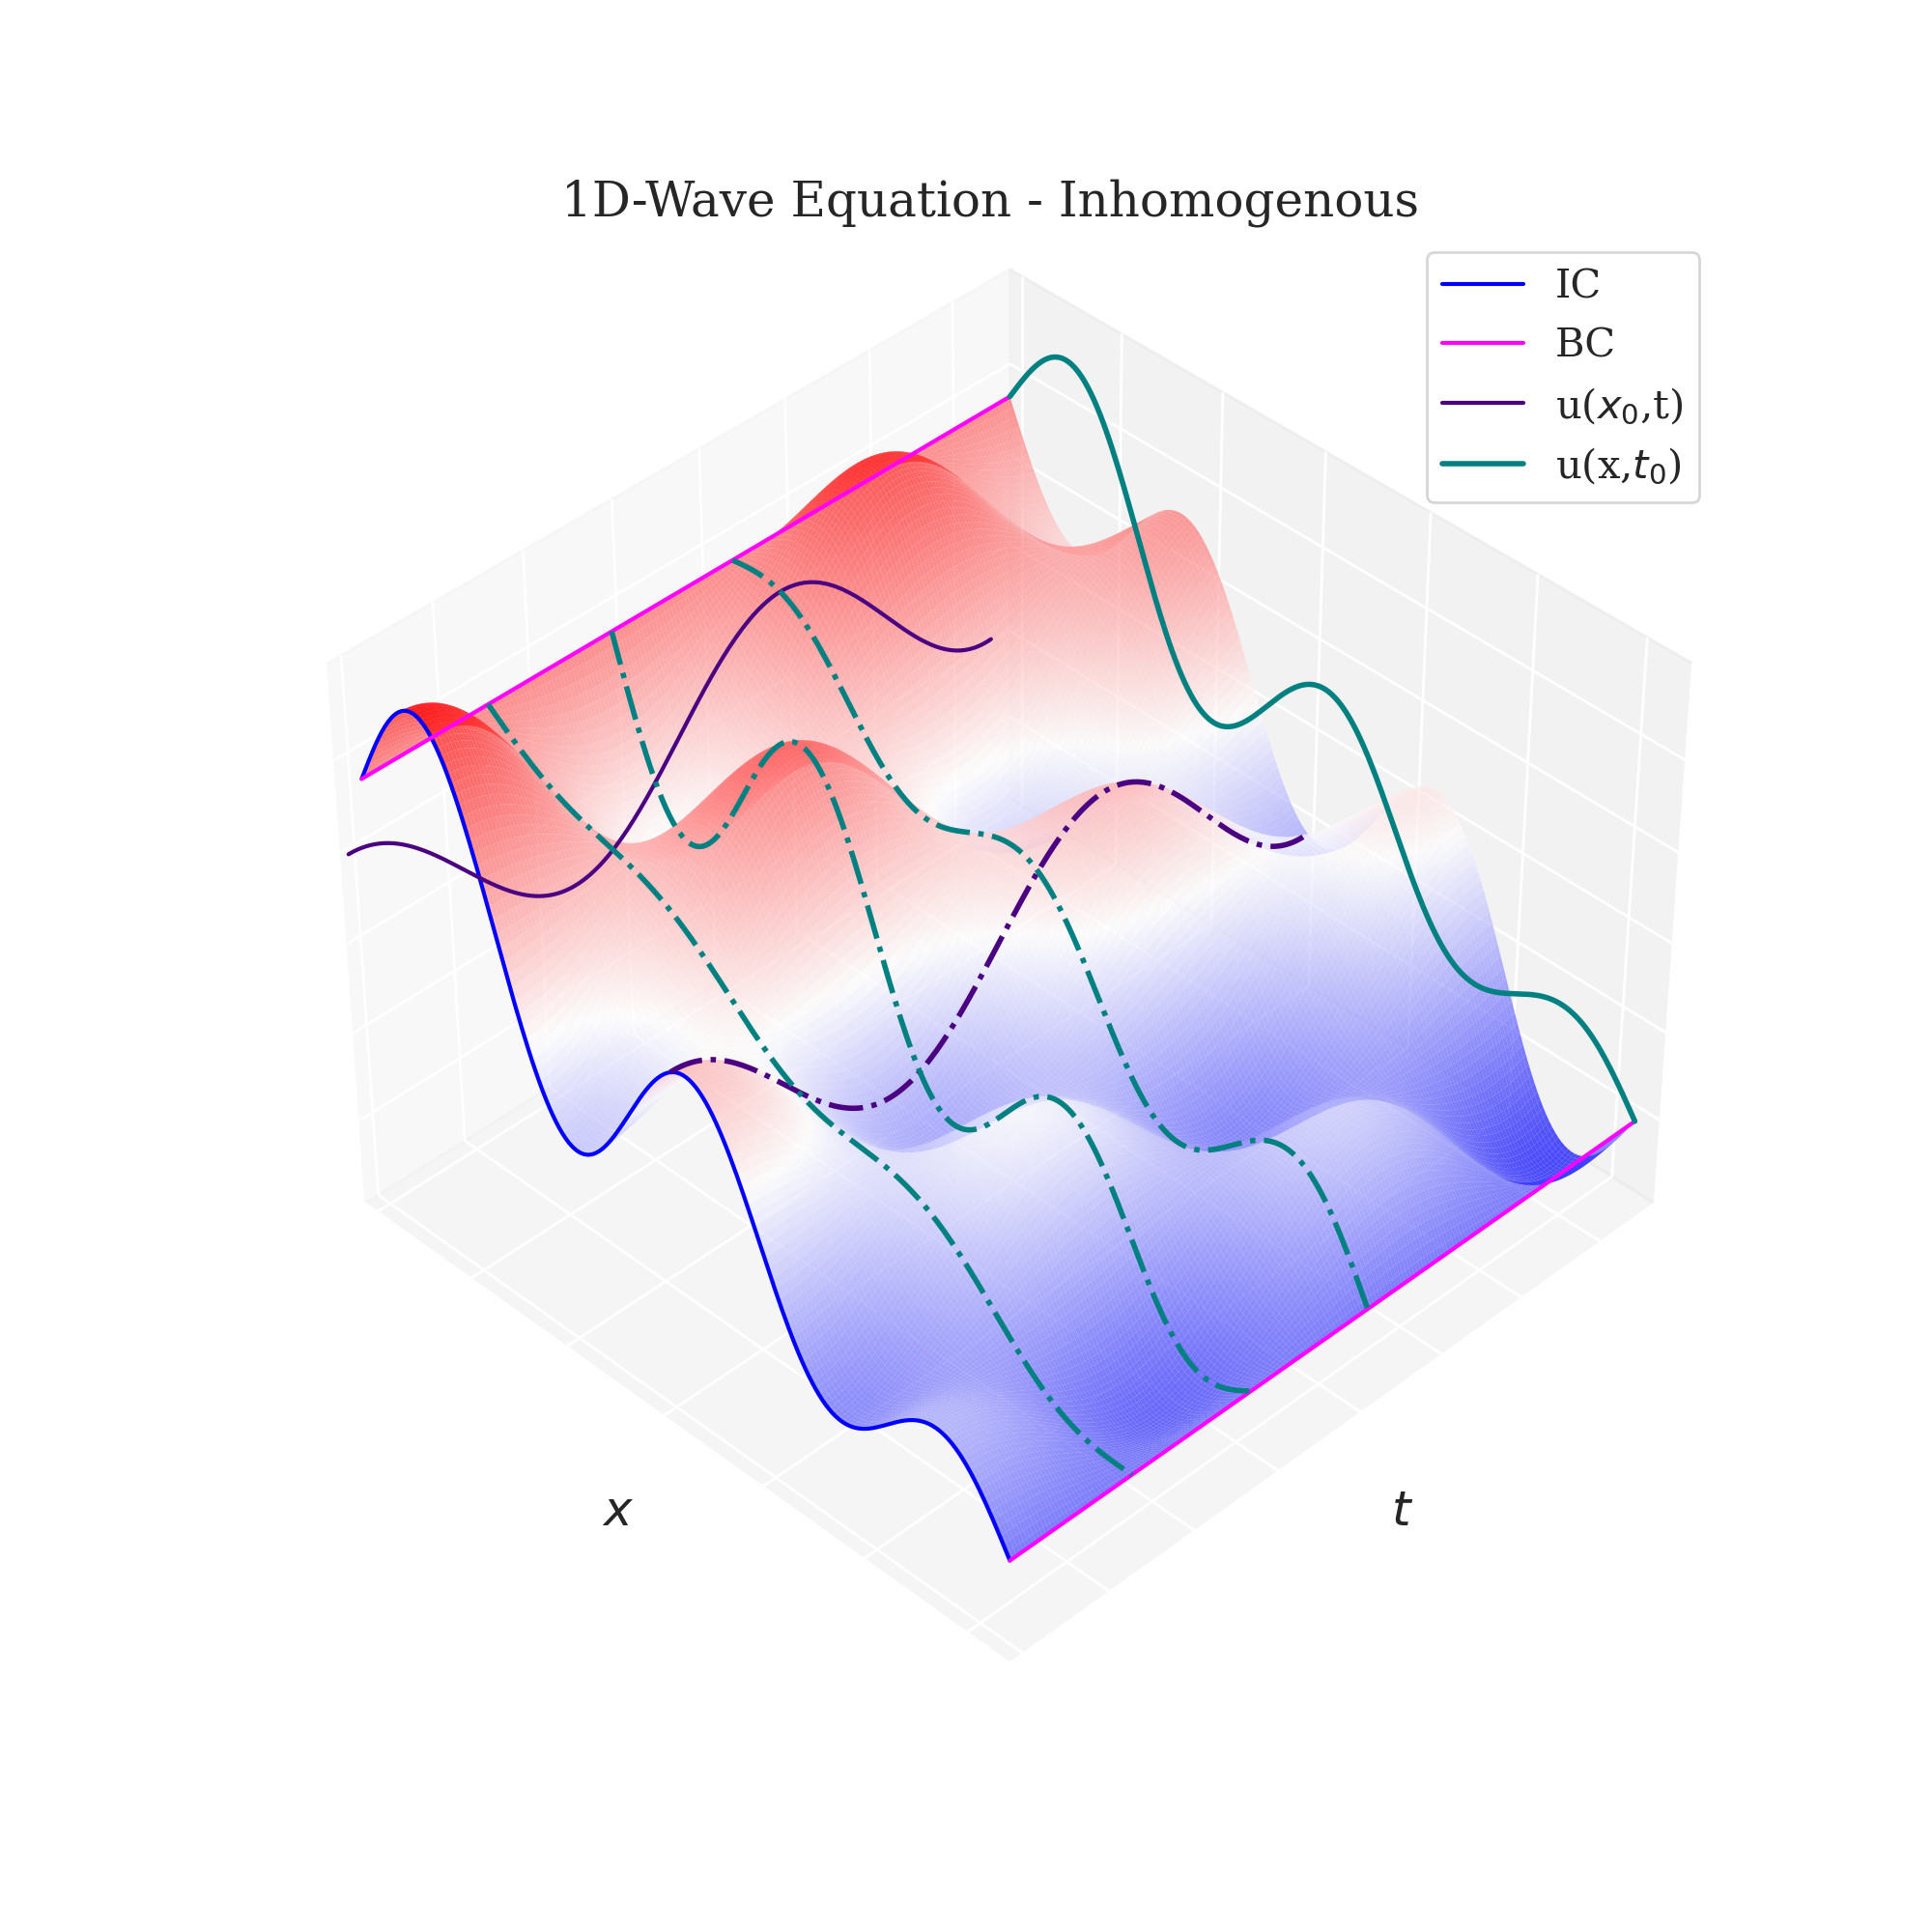
\includegraphics[width=0.85\linewidth]{../images/1d_wave_inhom.png}\\
\includegraphics[width=0.85\linewidth]{../images/1d_wave_fs.png}\\
\includegraphics[width=0.85\linewidth]{../images/1d_heat_fs.png}\\
\includegraphics[width=0.85\linewidth]{../images/2d_laplace.png}
    \newpage
    \section{Appendix}

\createsectiontoc{}

\subsection{Trigonometry}
\subsubsection{Common angles}
\begin{center}
    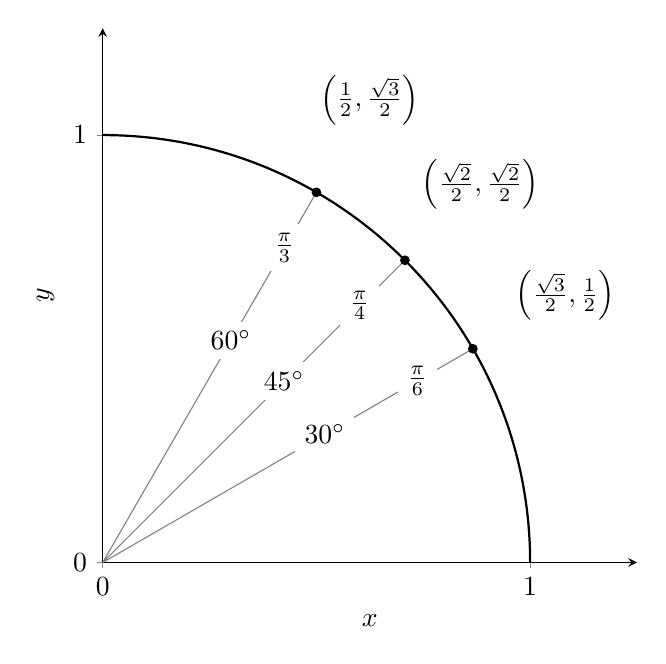
\begin{tikzpicture}
        \begin{axis}[
                width=0.8\linewidth,
                unit vector ratio={1 1},
                axis x line=left,
                axis y line=left,
                xmin=0,
                xmax=1.25,
                ymin=0,
                ymax=1.25,
                xlabel={$x$},
                ylabel={$y$},
                xtick={0, 1},
                ytick={0, 1},
                mark=none,
            ]
            \draw[thick] (0,0) circle(1);

            \draw[gray] \foreach \i in {30,45,60} {(0,0) -- ({cos(\i)},{sin(\i)})};
            \filldraw[black] \foreach \i in {30,45,60} {(\i:1) circle(0.01)};
            \draw \foreach \i in {30,45,60} {(\i:0.6) node[fill=white] {$\i^\circ$}};
            \draw \foreach \i/\itext in {30/\frac{\pi}{6},45/\frac{\pi}{4},60/\frac{\pi}{3}} {(\i:0.85) node[fill=white] {$\itext$}};

            \draw \foreach \i/\itext/\y in {
                    30/\frac{\sqrt{3}}{2}/\frac{1}{2},
                    45/\frac{\sqrt{2}}{2}/\frac{\sqrt{2}}{2},
                    60/\frac{1}{2}/\frac{\sqrt{3}}{2}} {(\i:1.25) node[fill=white] {$\left(\itext,\y\right)$}};
        \end{axis}
    \end{tikzpicture}
\end{center}

\subsubsection{Identities}
Given: $n, j \in \mathbb{N}$
\begin{align*}
     & \sin(\pi n)                                                                                 & = & \: 0                                                       \\
     & \cos(\pi n)                                                                                 & = & \: {(-1)}^n                                                \\
     & \sin\left(\frac{\pi}{2}n\right) = \left(\frac{1 + {(-1)}^n}{2}\right){(-1)}^{\frac{n+2}{2}} & = & \begin{cases} 0 &n=2j \\ {(-1)}^j&n=2j+1 \end{cases}       \\
     & \sin\left(\frac{3\pi}{2}n\right)                                                            & = & \begin{cases} 0 &n=2j \\ {(-1)}^{j+1}&n:\, odd \end{cases} \\
     & \cos\left(\frac{\pi}{2}n\right) = \left(\frac{1+{(-1)}^n}{2}\right){(-1)}^{\frac{n}{2}}     & = & \begin{cases} {(-1)}^j &n=2j \\ 0 &n=2j+1 \end{cases}      \\
     & \cos\left(\frac{3\pi}{2}n\right)                                                            & = & \begin{cases} {(-1)}^{j} &n=2j \\ 0 &n=2j+1 \end{cases}    \\
     & \sin\left(\left(n\pm 1\right)\frac{\pi}{2}\right)                                           & = & \pm \cos\left(\frac{n\pi}{2}\right)                        \\
     & \cos\left(\left(n\pm 1\right)\frac{\pi}{2}\right)                                           & = & \mp \sin\left(\frac{n\pi}{2}\right)                        \\
     & \sin(90^\circ\pm\alpha) = \sin(\frac{\pi}{2} \pm \alpha)                                    & = & \cos(\alpha)                                               \\
     & \cos(90^\circ\pm\alpha) = \cos(\frac{\pi}{2} \pm \alpha)                                    & = & \mp\sin(\alpha)                                            \\
     & \sin(180^\circ\pm\alpha) = \sin(\pi \pm \alpha)                                             & = & \mp\sin(\alpha)                                            \\
     & \cos(180^\circ\pm\alpha) = \cos(\pi \pm \alpha)                                             & = & -\cos(\alpha)                                              \\
     & \frac{1}{\sin^2 \alpha}                                                                     & = & 1+\cot^2 (\alpha)                                          \\
     & \frac{1}{\cos^2 \alpha}                                                                     & = & 1+\tan^2 (\alpha)                                          \\
     & {(-1)}^n+{(-1)}^{-n}=e^{in\pi}+e^{-in\pi}                                                   & = & 2\cos(\pi n)                                               \\
     & {(-1)}^n-{(-1)}^{-n}=e^{in\pi}-e^{-in\pi}                                                   & = & 2i\sin(\pi n)
\end{align*}

\subsubsection{Goniometry}
\noindent
\begin{align*}
    \sin(x\pm y) & =\sin(x)\cos(y)\pm\cos(x)\sin(y)              \\
    \cos(x\pm y) & =\cos(x)\cos(y)\mp\sin(x)\sin(y)              \\
    \tan(x\pm y) & =\frac{\tan(x)\pm\tan(y)}{1\mp\tan(x)\tan(y)}
\end{align*}
\begin{align*}
    \sin(2x)                     & =2\sin(x)\cos(x)                         \\
    \cos(2x)=\cos^2(x)-\sin^2(x) & =1-2\sin^2(x)=2\cos^2(x)-1               \\
    \tan(2x)                     & =\frac{2\tan(x)}{1-\tan^2(x)}            \\
    \sin(3x)                     & =3\sin(x)-4\sin^3(x)                     \\
    \cos(3x)                     & =4\cos^3(x)-3\cos(x)                     \\
    \tan(3x)                     & =\frac{3\tan(x)-\tan^3(x)}{1-3\tan^2(x)}
\end{align*}
\begin{align*}
    \sin^2\left(\frac x2\right)    & =\frac{1-\cos(x)}{2}                                 \\
    \cos^2\left(\frac x2\right)    & =\frac{1+\cos(x)}{2}                                 \\
    \tan^2\left(\frac{x}{2}\right) & =\frac{1-\cos(x)}{1+\cos(x)}                         \\
    \tan\left(\frac x2\right)      & =\frac{1-\cos(x)}{\sin(x)}=\frac{\sin(x)}{1+\cos(x)}
\end{align*}
\begin{align*}
    \sin(x)\cos(y)      & =\frac12\Bigl[\sin(x+y)\;+\;\sin(x-y)\Bigr] \\
    \sin(x)\sin(y)      & =\frac12\Bigl[\cos(x-y)\;-\;\cos(x+y)\Bigr] \\
    \cos(x)\cos(y)      & =\frac12\Bigl[\cos(x+y)\;+\;\cos(x-y)\Bigr] \\
    \sin(x)\pm\sin(y)   & =2\sin\frac{x\pm y}{2}\cos\frac{x \mp y}{2} \\
    \cos(x)+\cos(y)     & =2\cos\frac{x+y}{2}\cos\frac{x-y}{2}        \\
    \cos(x)-\cos(y)     & =-2\sin\frac{x+y}{2}\sin\frac{x-y}{2}       \\
    \tan(x) \pm \tan(y) & = \frac{\sin(x\pm y)}{\cos(x)\cos(y)}
\end{align*}

\subsubsection{Transformations}

\renewcommand{\arraystretch}{1.3}

\setlength\tabcolsep{6pt} % default value: 6pt

\begin{tabularx}{\linewidth}{@{}p{0.15\linewidth}ccc@{}}
                                                    & $\sin$                                         & $\cos$                                         & $\tan$                                         \\
    \cmidrule{2-4}
    $\sin(\alpha)=$                                 &                                                & $\sqrt{1-\cos^2(\alpha)}$                      & $\frac{\tan(\alpha)}{\sqrt{1+\tan^2(\alpha)}}$ \\
    $\cos(\alpha)=$                                 & $\sqrt{1-\sin^2(\alpha)}$                      &                                                & $\frac{1}{\sqrt{1+\tan^2(\alpha)}}$            \\
    $\tan(\alpha)=$ \newline $\alpha \neq 90^\circ$ & $\frac{\sin(\alpha)}{\sqrt{1-\sin^2(\alpha)}}$ & $\frac{\sqrt{1-\cos^2(\alpha)}}{\cos(\alpha)}$ &
\end{tabularx}

\renewcommand{\arraystretch}{1}

\setlength\tabcolsep{6pt} % default value: 6pt

\subsubsection{Euler-Relation}
\noindent
\begin{align*}
    \sin(x)    & =\frac{1}{2i}(e^{ix}-e^{-ix})             \\
    \cos(x)    & =\frac{1}{2}(e^{ix}+e^{-ix})              \\
    \tan(x)    & =\frac{e^{ix}-e^{-ix}}{i(e^{ix}+e^{-ix})} \\
    \sinh(x)   & =\frac{1}{2}(e^{x}-e^{-x})                \\
    \cosh(x)   & =\frac{1}{2}(e^{x}+e^{-x})                \\
    \tanh(x)   & =\frac{e^{x}-e^{-x}}{(e^{x}+e^{-x})}      \\
    e^{ix}     & = \cos(x) + i \cdot \sin(x)               \\
    e^{k\pi i} & = \begin{cases}
                       1  & k = 2n     \\
                       -1 & k = 2n + 1
                   \end{cases} \quad n \in \mathbb{N}
\end{align*}

\subsubsection{Inverse functions}
\noindent
\begin{align*}
    \sin(\arccos(x))                         & = \sqrt{1-x^2}                                                 \\
    \cos(\arcsin(x))                         & =\sqrt{1-x^2}                                                  \\
    \sin(\arctan(x))                         & =\frac{x}{\sqrt{x^2+1}}                                        \\
    \cos(\arctan(x))                         & =\frac{1}{\sqrt{x^2+1}}                                        \\
    \tan(\arcsin(x))                         & =x \cdot {(1-x)}^{-\frac{1}{4}}                                \\
    \tan(\arccos(x))                         & =x^{-1} \cdot {(1-x)}^{\frac{1}{4}}                            \\
    \operatorname{arcsinh}(x)                & =\ln(x+\sqrt{x^2+1})                                           \\
    \operatorname{arccosh}(x)                & =\ln(x+\sqrt{x^2-1})                                           \\
    \operatorname{arctanh}(x)                & =\frac{1}{2}\cdot \ln(\frac{1+x}{1-x}); \quad \vert x\vert < 1 \\
    \operatorname{arccoth}(x)                & =\frac{1}{2}\cdot \ln(\frac{1+x}{x-1}); \quad \vert x\vert > 1 \\
    \sinh(2 \cdot \operatorname{arcsinh}(x)) & =2x\sqrt{x^2-1}                                                \\
    \sinh(\operatorname{arccosh}(x))         & =\sqrt{x^2-1};\qquad x>0                                       \\
    \cosh(\operatorname{arcsinh}(x))         & =\sqrt{x^2+1}
\end{align*}

\subsection{Derivatives}

\textbf{Sums and Constants}
\begin{align*}
    (f\pm g)'             & =f'\pm g'                                  \\
    {(c\cdot f)}^{\prime} & =c\cdot f^{\prime}\quad(c\text{ constant})
\end{align*}

\textbf{Product/ Quotient Rule}
\begin{align*}
    (f\cdot g)'                      & =f'\cdot g+f\cdot g'                             \\
    {\left(\frac fg\right)}^{\prime} & =\frac{f^{\prime}\cdot g-f\cdot g^{\prime}}{g^2}
\end{align*}

\textbf{Reciprocal Rule}
\begin{align*}
    {\left(\frac{1}{f}\right)}^{\prime} & = -\frac{f^{\prime}}{f^2}
\end{align*}

\textbf{Chain Rule}
\begin{align*}
    {[f(g(x))]}^{\prime}          & =f^{\prime}(g(x))\cdot g^{\prime}(x)                         \\
    F'(t)                         & =f_x(x(t),y(t))\cdot\dot{x}(t)+f_y(x(t),y(t))\cdot\dot{y}(t) \\
    \frac{\partial y}{\partial x} & = \frac{\partial y}{\partial u}\frac{\partial u}{\partial x}
\end{align*}

\subsubsection{Common Derivatives}
\noindent
\begin{align*}
     & \frac{d}{dx}x^n                       &  & =nx^{n-1}                              \\
     & \frac{d}{dx}e^x                       &  & =e^x                                   \\
     & \frac{d}{dx}a^x                       &  & =a^x\ln(a),\quad a>0                   \\
     & \frac{d}{dx}\ln(x)                    &  & =\frac1x                               \\
     & \frac{d}{dx}\log_a(x)                 &  & =\frac1{x\ln(a)}                       \\
     & \frac{d}{dx}\sin(x)                   &  & =\cos(x)                               \\
     & \frac{d}{dx}\cos(x)                   &  & =-\sin(x)                              \\
     & \frac{d}{dx}\tan(x)                   &  & =\frac1{\cos^2(x)}=1+\tan^2(x)         \\
     & \frac{d}{dx}\arcsin(x)                &  & =\frac1{\sqrt{1-x^2}}                  \\
     & \frac{d}{dx}\arccos(x)                &  & =-\frac1{\sqrt{1-x^2}}                 \\
     & \frac{d}{dx}\arctan(x)                &  & =\frac1{1+x^2}                         \\
     & \frac{d}{dx}\sinh(x)                  &  & =\cosh(x)                              \\
     & \frac{d}{dx}\cosh(x)                  &  & =\sinh(x)                              \\
     & \frac{d}{dx}\tanh(x)                  &  & =\frac{1}{\cosh^{2}(x)}=1-\tanh^{2}(x) \\
     & \frac{d}{dx}\sinh(x)                  &  & =\frac1{\sqrt{x^2+1}}                  \\
     & \frac{d}{dx}\operatorname{arccosh}(x) &  & =\frac1{\sqrt{x^2-1}}                  \\
     & \frac{d}{dx}\operatorname{arctanh}(x) &  & =\frac1{1-x^2}
\end{align*}

\subsection{Integral calculus}
\textbf{Hauptsatz}
\begin{align*}
    F^{\prime}(x) & =f(x)\Longrightarrow\int_a^b f(x)dx=F(b)-F(a)
\end{align*}

\textbf{Sums and Constants}
\begin{align*}
    \int_a^b\left(f\pm g\right)dx & =\int_a^b f\;dx\pm\int_a^b g\;dx         \\
    \int_a^b c\cdot f\;dx         & =c\int_a^b f\;dx\quad(c\text{ constant})
\end{align*}

\textbf{Partial Integration}
\begin{align*}
     & \int_a^b f'\cdot g\left.dx=(f\cdot g)\right|_a^b-\int_a^b f\cdot g'\;dx        \\
     & \int_a^b f\cdot g\left.dx=(F\cdot g)\right|_a^b-\int_a^b F\cdot g^{\prime}\;dx
\end{align*}

\textbf{Substitution}
\begin{align*}
     & \text{Substitution }u=g(x){:}                                          \\
     & \int_a^b f(g(x))g^{\prime}(x)\;dx=\int_{g(a)}^{g(b)}f(u)\;du           \\\\
     & \text{Substitution }x=g(y){:}                                          \\
     & \int_a^b f(x)\;dx=\int_{g^{-1}(a)}^{g^{-1}(b)}f(g(y))g^{\prime}(y)\;dy
\end{align*}

\textbf{Common Substitutions}:\par

\renewcommand{\arraystretch}{1.3}

\begin{tabularx}{\linewidth}{@{}lll@{}}
    Integral               & Subst.                        & Comment                                    \\
    \cmidrule{1-3}
    $f(ax+b)$              & $t=ax+b$                      &                                            \\
    $f(g(x))g^{\prime}(x)$ & $g(x)=t$                      & $=\int f(t)dt$                             \\
    $f(x,\sqrt{ax+b})$     & $x=\frac{t^2-b}{a}$           & $t\geq0$                                   \\
    $f(x,\sqrt{a^2-x^2})$  & $x=\arcsin(t)$                & $\sqrt{a^2-x^2}=\operatorname{arccosh}(t)$ \\
    $f(x,\sqrt{x^2-a^2})$  & $x=\operatorname{arccosh}(t)$ & $\sqrt{x^2-a^2}=\operatorname{arcsinh}(t)$ \\
    $f(\sin(x),\cos(x))$   & $t=\tan(\frac {x}{2})$        & $\sin(x)=\frac{2t}{1+t^2}$                 \\
                           &                               & $\cos(x)=\frac{1-t^2}{1+t^2}$              \\
                           &                               & $dx=\frac{2dt}{1+t^2}$                     \\
    $f(e^x,\sinh,\cosh)$   & $t=e^x$                       & $\sinh(x)=\frac{t^2-1}{2t}$                \\
\end{tabularx}

\renewcommand{\arraystretch}{1}


\subsubsection{Integration of trigonometric functions}
\noindent
\begin{small}
    \begin{align*}
         & \int \sin(x) dx                  &  & = -\cos(x) + C                                                  \\
         & \int \cos(x) dx                  &  & = \sin(x) + C                                                   \\
         & \int \tan(x) dx                  &  & = -\ln\vert\cos(x)\vert +C                                      \\
         & \int \cot(x)dx                   &  & = \ln\vert\sin(x)\vert +C                                       \\
         & \int \sin^2(ax) dx               &  & = \frac{x}{2}-\frac{\sin(2ax)}{4a}+C                            \\
         & \int \cos^2(ax) dx               &  & = \frac{x}{2}+\frac{\sin(2ax)}{4a}+C                            \\
         & \int \tan^2(ax) dx               &  & = \frac{1}{a}(-ax+\tan(ax))+C                                   \\
         & \int \sin^3(x)dx                 &  & = \frac{1}{12}(\cos(3x)-9\cos(x))+C                             \\
         & \int \cos^3(x)dx                 &  & = \frac{1}{12}(9\sin(x)+\sin(3x))+C                             \\
         & \int \tan^3(x)dx                 &  & = \frac{\sec^2(x)}{2}+\ln(\cos(x))+C                            \\
         & \int \sin^4(x)dx                 &  & = \frac{1}{32}(12x-8\sin(2x)+\sin(4x))+C                        \\
         & \int \cos^4(x)dx                 &  & = \frac{1}{32}(12x+8\sin(2x)+\sin(4x))+C                        \\
         & \int \tan^4(x)dx                 &  & = x+\frac{1}{3}\tan(x)(\sec^2(x)-4)+C                           \\
         & \int \sin^n(x) dx                &  & = -\frac{1}{n}\sin^{n-1}(x)\cos(x) \dots                        \\
         &                                  &  & \qquad +\frac{n-1}{n}\int \sin^{n-2}(x) dx; \quad n\geq 2       \\
         & \int \cos^n(x) dx                &  & = \frac{1}{n}\sin(x)\cos^{n-1}(x) \dots                         \\
         &                                  &  & \qquad +\frac{n-1}{n}\int \cos^{n-2}(x) dx; \quad n\geq 2       \\
         & \int \sin^{\frac{3}{2}}(2x) dx   &  & = -\frac{1}{2}\cos(2x)+C                                        \\
         & \int \cos^{\frac{3}{2}}(2x) dx   &  & = \sin(x)\cos(x)+C                                              \\
         & \int x \cdot \sin(ax) dx         &  & = \frac{\sin(ax)}{a^2}-\frac{x \cdot \cos(ax)}{a}+C             \\
         & \int x \cdot \cos(ax) dx         &  & = \frac{\cos(ax)}{a^2}+\frac{x \cdot \sin(ax)}{a}+C             \\
         & \int x^2 \sin(ax) dx             &  & = \frac{1}{a^3} [-a^2x^2\cos(ax) + 2 \cdot \cos(ax) \dots       \\
         &                                  &  & \qquad + 2 ax \sin(ax)]+C                                       \\
         & \int x^2 \cos(ax) dx             &  & = \frac{1}{a^3} [a^2x^2\sin(ax) - 2 \cdot \sin(ax) \dots        \\
         &                                  &  & \qquad + 2ax \cos(ax)]+C                                        \\
         & \int e^x \sin(x) dx              &  & = \frac{e^x}{2}(\sin(x) - \cos(x))+C                            \\
         & \int e^x \cos(x) dx              &  & = \frac{e^x}{2}(\sin(x) + \cos(x))+C                            \\
         & \int e^{ax} \sin(bx)dx           &  & = \frac{e^{ax}}{a^2+b^2}[a\cdot \sin(bx)+b\cdot \cos(bx)]+C     \\
         & \int e^{ax} \cos(bx)dx           &  & = \frac{e^{ax}}{a^2+b^2}[a\cdot \cos(bx)+b\cdot \sin(bx)]+C     \\
         & \int \frac{1}{\sin(x)}dx         &  & = \ln\left| \tan\frac{x}{2}\right| +C                           \\
         & \int \frac{1}{\cos(x)}dx         &  & = \ln\left| \tan\left(\frac{x}{2}+\frac{\pi}{4}\right)\right|+C \\
         & \int \frac{2}{\tan(x)}dx         &  & = \ln\vert \sin\; x\vert +C                                     \\
         & \int \frac{1}{\sin^2(x)}dx       &  & = -\cot(x)+C                                                    \\
         & \int \frac{1}{\cos^2(x)}dx       &  & = \tan(x)+C                                                     \\
         & \int \tan(ax) dx                 &  & = -\frac{1}{a} \cdot \ln{\mid \cos(ax) \mid }+C                 \\
         & \int \arcsin (x) dx              &  & = x \cdot \arcsin(x)+\sqrt{1-x^2}+C                             \\
         & \int \arccos (x) dx              &  & = x \cdot \arccos(x)-\sqrt{1-x^2}+C                             \\
         & \int \arctan (x) dx              &  & = x \cdot \arctan(x)-\frac{1}{2} \cdot \ln(1+x^2)+C             \\
         & \int \sinh(x)dx                  &  & = \cosh(x)+C                                                    \\
         & \int \cosh(x)dx                  &  & = \sinh(x)+C                                                    \\
         & \int \tanh(x)dx                  &  & = \ln(\cosh(x)) +C                                              \\
         & \int \coth(x)dx                  &  & = \ln(\sinh(x))+C                                               \\
         & \int \operatorname{arcsinh}(x)dx &  & = x \cdot \operatorname{arcsinh}(x) - \sqrt{x^2+1}+C            \\
         & \int \operatorname{arccosh}(x)dx &  & = x \cdot \operatorname{arccosh}(x) - \sqrt{x^2-1}+C            \\
         & \int \operatorname{arctanh}(x)dx &  & = x \cdot \operatorname{arctanh}(x) +\frac{1}{2}\ln(1-x^2)+C
    \end{align*}
    \begin{align*}
         & \int \sin(ax)\cos(ax) dx           &  & = -\frac{\cos^2(ax)}{2a}+C                 \\
         & \int \sin^2(x)\cos(x)dx            &  & =\frac{1}{3}\sin^3(x)+C                    \\
         & \int \sin(x)\cos^2(x)dx            &  & =-\frac{1}{3}\cos^3(x)+C                   \\
         & \int \sin^2(x)\cos^2(x)dx          &  & =\frac{1}{32}(4x-\sin(4x))+C               \\
         & \int \sin^n(ax)\cdot \cos(ax)dx    &  & =\frac{\sin^{n+1}(ax)}{(n+1)a}+C           \\
         & \int \sin(ax)\cdot \cos^n(ax)dx    &  & =-\frac{\cos^{n+1}(ax)}{(n+1)a}+C          \\
         & \int \frac{\cos(ax)}{\sin^n(ax)}dx &  & = -\frac{1}{(n-1)a \cdot \sin^{n-1}(ax)}+C
    \end{align*}
\end{small}

\subsubsection{Integration of trig.\ functions on special intervals}
\noindent
\begin{align*}
    \int_{-L}^L \cos\left(\frac{n\pi x}{L}\right)\cdot \cos\left(\frac{m\pi x}{L}\right) dx & =\begin{cases}
                                                                                                   0  & \text{if } n\neq m \\
                                                                                                   L  & \text{if } n=m     \\
                                                                                                   2L & \text{if } n=m=0
                                                                                               \end{cases}  \\
    \int_{-L}^L \sin\left(\frac{n\pi x}{L}\right)\cdot \sin\left(\frac{m\pi x}{L}\right) dx & =\begin{cases}
                                                                                                   0 & \text{if }n\neq m    \\
                                                                                                   L & \text{if } n=m\neq 0
                                                                                               \end{cases} \\
    \int_{-L}^L \sin\left(\frac{n\pi x}{L}\right)\cdot \cos\left(\frac{m\pi x}{L}\right) dx & =0\;\;\forall\; n,m
\end{align*}
\begin{align*}
    \sin(nx)\Big|_0^{2\pi}  & =0 &  & \cos(nx)\Big|_0^{2\pi}=0          \\
    x\sin(nx)\Big|_0^{2\pi} & =0 &  & x\cos(nx)\Big|_0^{2\pi}=2\pi\neq0
\end{align*}
\begin{align*}
     & \int_0^{\infty} \frac{\sin(ax)}{x} dx &  & =\frac{\pi}{2};\quad a>0                                                 \\
     & \int_0^{\infty} \sin(x^2) dx          &  & =\int_0^{\infty}\cos(x^2)dx=\frac{1}{2}\sqrt{\frac{\pi}{2}}              \\
     & \int_{-\pi}^{\pi} e^{ijx} \text{d}x   &  & = \begin{cases}2\pi & \text{if } j=0\\ 0 & \text{if } j\neq 0\end{cases}
\end{align*}


\renewcommand{\arraystretch}{1.5}

\setlength\tabcolsep{8pt} % default value: 6pt

\begin{tabularx}{\linewidth}{@{}lccccccc@{}}
                        & $\int\limits_0^{\frac{\pi}{4}} $ & $\int\limits_0^{\frac{\pi}{2}}$ & $\int\limits_0^{\pi}$ & $\int\limits_0^{2\pi}$ & $\int\limits_{-\frac{\pi}{4}}^{\frac{\pi}{4}} $ & $\int\limits_{-\frac{\pi}{2}}^{\frac{\pi}{2}} $ & $\int\limits_{-\pi}^{\pi}$ \\
    \cmidrule{2-8}
    $\sin$              & $\frac{\sqrt{2}-1}{\sqrt{2}}$    & 1                               & 2                     & 0                      & 0                                               & 0                                               & 0                          \\
    $\sin^2$            & $\frac{\pi-2}{8}$                & $\frac{\pi}{4}$                 & $\frac{\pi}{2}$       & $\pi$                  & $\frac{\pi-2}{4}$                               & $\frac{\pi}{2}$                                 & $\pi$                      \\
    $\sin^3$            & $\frac{8-5\sqrt{2}}{12}$         & $\frac{2}{3}$                   & $\frac{4}{3}$         & 0                      & 0                                               & 0                                               & 0                          \\
    $\sin^4$            & $\frac{3\pi-8}{32}$              & $\frac{3\pi}{16}$               & $\frac{3\pi}{8}$      & $\frac{3\pi}{4}$       & $\frac{3\pi-8}{16}$                             & $\frac{3\pi}{8}$                                & $\frac{3\pi}{4}$           \\
    $\cos$              & $ \frac{1}{\sqrt{2}}$            & 1                               & 0                     & 0                      & $\sqrt{2}$                                      & 2                                               & 0                          \\
    $\cos^2$            & $\frac{2+\pi}{8}$                & $\frac{\pi}{4}$                 & $\frac{\pi}{2}$       & $\pi$                  & $\frac{2+\pi}{4}$                               & $\frac{\pi}{2}$                                 & $\pi$                      \\
    $\cos^3$            & $\frac{5}{6\sqrt{2}}$            & $\frac{2}{3}$                   & 0                     & 0                      & $\frac{5}{3\sqrt{2}}$                           & $\frac{4}{3}$                                   & 0                          \\
    $\cos^4$            & $\frac{8+3\pi}{32}$              & $\frac{3\pi}{16}$               & $\frac{3\pi}{8}$      & $\frac{3\pi}{4}$       & $\frac{8+3\pi}{16}$                             & $\frac{3\pi}{8}$                                & $\frac{3\pi}{4}$           \\
    $\sin \cdot \cos$   & $\frac{1}{4}$                    & $\frac{1}{2}$                   & 0                     & 0                      & 0                                               & 0                                               & 0                          \\
    $\sin^2 \cdot \cos$ & $\frac{1}{6\sqrt{2}}$            & $\frac{1}{3}$                   & 0                     & 0                      & $\frac{1}{3\sqrt{2}}$                           & $\frac{2}{3}$                                   & 0                          \\
    $\sin \cdot \cos^2$ & $\frac{4-\sqrt{2}}{12}$          & $\frac{1}{3}$                   & $\frac{2}{3}$         & 0                      & 0                                               & 0                                               & 0
\end{tabularx}

\renewcommand{\arraystretch}{1}

\setlength\tabcolsep{6pt} % default value: 6pt

\subsubsection{Intergation of power, rational, exponential and logarithmic functions}
\noindent
\begin{footnotesize}
    \begin{align*}
         & \int {(ax+b)}^n dx                    &  & =\frac{{(ax+b)}^{n+1}}{(n+1)a}+C                                                  \\
         & \int x{(ax+b)}^n dx                   &  & =\frac{{(ax+b)}^{n+2}}{(n+2)a^2}-\frac{b{(ax+b)}^{n+1}}{(n+1)a^2}+C               \\
         & \int x^2{(ax+b)}^n dx                 &  & =\frac{{(ax+b)}^{n+3}}{(n+3)a^3}-\frac{2b{(ax+b)}^{n+2}}{(n+2)a^3} \dots          \\
         &                                       &  & \qquad +\frac{b^2{(ax+b)}^{n+1}}{(n+1)a^3}+C                                      \\
         & \int \frac{1}{ax+b}dx                 &  & =\frac{1}{a}\ln\vert ax+b \vert +C                                                \\
         & \int \frac{ax+b}{cx+d}dx              &  & =\frac{ax}{c}-\frac{ad-bc}{c^2}\ln\vert cx+d \vert +C                             \\
         & \int \frac{x}{{(ax+b)}^n}dx           &  & =-\frac{1}{(n-2)a^2{(ax+b)}^{n-2}} \dots                                          \\
         &                                       &  & \qquad +\frac{b}{(n-1)a^2{(ax+b)}^{n-1}}+C                                        \\
         & \int \frac{x}{x^2+a}dx                &  & =\frac{1}{2}\ln\vert x^2+a \vert+C                                                \\
         & \int \frac{x}{ax^2+b}dx               &  & =\frac{1}{2a}\ln \vert ax^2+b \vert+C                                             \\
         & \int \frac{1}{x^2-a^2}dx              &  & =\frac{1}{2a}\ln \vert \frac{x-a}{x+a}\vert+C                                     \\
         & \int \frac{1}{x^2+a^2}dx              &  & =\frac{1}{a}\arctan(\frac{x}{a})+C                                                \\
         & \int \frac{x}{{(x^2+a^2)}^n}dx        &  & =-\frac{1}{2(n-1){(a^2+x^2)}^{n-1}}+C                                             \\
         & \int \frac{x}{{(a^2-x^2)}^n}dx        &  & =\frac{1}{2(n-1){(a^2-x^2)}^{n-1}}+C                                              \\
         & \int \frac{x^2-a^2}{x^2+a^2}dx        &  & =\frac{a}{x^2+a^2}+C                                                              \\
         & \int {(ax^p+b)}^s x^{p-1}dx           &  & =\frac{{(ax^p+b)}^{s+1}}{ap(s+1)}+C,\quad s\neq -1,\; a, p\neq 0                  \\
         & \int {(ax^p+b)}^{-1}x^{p-1}dx         &  & =\frac{1}{ap}\ln\vert ax^p+b\vert +C,\quad a\neq 0,\; p\neq 0                     \\
         & \int \sqrt{a^2+x^2}dx                 &  & =\frac{x}{2}\sqrt{a^2+x^2}+\frac{a^2}{2}\ln(x+\sqrt{a^2+x^2})+C                   \\
         & \int \sqrt{a^2-x^2}dx                 &  & =\frac{x}{2}\sqrt{a^2-x^2}+\frac{a^2}{2}\arcsin\frac{x}{\vert a \vert}+C          \\
         & \int \sqrt{x^2-a^2}dx                 &  & =\frac{x}{2}\sqrt{x^2-a^2}-\frac{a^2}{2}\ln\big\vert x+\sqrt{x^2-a^2}\big\vert +C \\
         & \int \frac{1}{\sqrt{x^2+a^2}}dx       &  & =\ln(x+\sqrt{a^2+x^2})+C                                                          \\
         & \int \frac{2}{\sqrt{x^2-a^2}}dx       &  & =\ln\vert x+\sqrt{x^2-a^2}\vert +C                                                \\
         & \int \frac{1}{\sqrt{a^2-x^2}}dx       &  & =\arcsin\frac{x}{\vert a\vert }+C                                                 \\
         & \int \frac{1}{x^2+x}dx                &  & =\ln(x)-\ln(x+1)+C                                                                \\
         & \int \frac{1}{ax^2+bx+c}dx            &  & =\frac{2\arctan(\frac{2ax+b}{\sqrt{4ac-b^2}})}{\sqrt{4ac-b^2}}+C                  \\
         & \int \frac{1}{\sqrt{1-x^2}}dx         &  & =\arcsin(x)+C                                                                     \\
         & \int \frac{-1}{\sqrt{1-x^2}}dx        &  & =\arccos(x)+C                                                                     \\
         & \int \frac{1}{1-x^2}dx                &  & =\operatorname{arctanh}(x)=\log(\sqrt{\frac{1+x}{1-x}})+C, \vert x \vert < 1      \\
         & \int \frac{1}{\sqrt{x^2+1}}dx         &  & =\operatorname{arcsinh}(x)=\log(x+\sqrt{x^2+1})+C                                 \\
         & \int \frac{1}{\sqrt{x^2-1}}dx         &  & =\operatorname{arccosh}(x)=\log(x+\sqrt{x^2-1})+C, 1 \leq x                       \\
         & \int e^{kx}dx                         &  & =\frac{1}{k}e^{kx}+C                                                              \\
         & \int a^{kx}dx                         &  & =\frac{1}{k\cdot \ln(a)}a^{kx}+C                                                  \\
         & \int e^{kx}\sin(ax+b)dx               &  & =\frac{e^{kx}}{a^2+k^2}\left(k\sin(ax+b)-a\cos(ax+b)\right)+C                     \\
         & \int e^{kx}\cos(ax+b)dx               &  & =\frac{e^{kx}}{a^2+k^2}\left(k\cos(ax+b)+a\sin(ax+b)\right)+C                     \\
         & \int x \cdot e^{ax}dx                 &  & =(\frac{ax-1}{a^2})\cdot e^{ax}+C                                                 \\
         & \int x^2 \cdot e^{ax}dx               &  & =(\frac{a^2x^2-2ax+2}{a^3})\cdot e^{ax}                                           \\
         & \int x\cdot e^{x^2}dx                 &  & =\frac{1}{2}\cdot e^{x^2}+C                                                       \\
         & \int \frac{1}{e^x+a}dx                &  & =\frac{x-\ln(a+e^x)}{a}+C                                                         \\
         & \int \frac{1}{e^x-a}dx                &  & =\frac{\ln(e^x-a)-x}{a}+C                                                         \\
         & \int \frac{1}{p+q\cdot e^{ax}}dx      &  & =\frac{x}{p}-\frac{1}{ap}\cdot \ln\vert p+q\cdot e^{ax}\vert+C                    \\
         & \int \frac{e^{ax}}{p+q\cdot e^{ax}}dx &  & =\frac{1}{ap}\cdot \ln\vert p+q\cdot e^{ax}\vert                                  \\
         & \int \ln\vert x\vert dx               &  & =x(\ln\vert x \vert -1)+C                                                         \\
         & \int \log_a\vert x \vert dx           &  & =x(\log_a\vert x\vert -\log_a e)+C                                                \\
         & \int x \cdot \ln(x) dx                &  & =\frac 1 2 \cdot x^2(\ln(x)-\frac{1}{2})+C                                        \\
         & \int x^k \ln\; x \;dx                 &  & =\frac{x^{k+1}}{k+1}\left(\ln\; x-\frac{1}{k+1}\right)+C,\quad k\neq -1           \\
         & \int c\ln(a)a^{cx}                    &  & = a^{cx} + C                                                                      \\
         & \int x^{-1}\ln\; x \; dx              &  & =\frac{1}{2}{(\ln\; x)}^2+C                                                       \\
         & \int \frac{{(\ln(x))}^n}{x}dx         &  & =\frac{{(\ln(x))}^{n+1}}{x+1}+C                                                   \\
         & \int \frac{1}{x\ln(a)}                &  & = \log_a|x| +C                                                                    \\
         & \int \frac{f'(x)}{f(x)}dx             &  & =\ln\vert f(x) \vert +C                                                           \\
         & \int f'(x) \cdot f(x) dx              &  & = \frac{1}{2}(f^2(x))+C
    \end{align*}
\end{footnotesize}

\subsubsection{Integration over special intervals}
\noindent
\begin{align*}
     & \int_{-\infty}^{\infty}\frac{1}{1+x^2}dx    &  & = \pi                                      \\
     & \int_0^{\infty} e^{-ax}x^n dx               &  & =\frac{n!}{a^{n+1}},\quad a>0              \\
     & \int_0^{\infty} e^{-ax^2} dx                &  & =\frac{1}{2}\sqrt{\frac{\pi}{a}},\quad a>0 \\
     & \int_{-\infty}^{\infty} e^{-ax^2} dx        &  & =\sqrt{\frac{\pi}{a}},\quad a>0            \\
     & \int_{-\infty}^{\infty}e^{-ax^2}e^{-iwx} dx &  & = \sqrt{\frac{\pi}{a}}e^{\frac{w^2}{4a}}   \\
     & \int_{-\infty}^{\infty}e^{-(ax^2+bx+c)}dx   &  & = \sqrt{\frac{\pi}{a}}e^{\frac{b^2}{4a}-c} \\
\end{align*}

\subsection{Various functions and their properties}
\subsubsection{even and odd functions}
\noindent
\begin{gather*}
    even \cdot even\;\widehat{=}\; odd \cdot odd \;\widehat{=}\; even \\
    even \cdot odd \;\widehat{=}\; odd \\
    \int\limits_{-L}^L even=2\int\limits_0^L even \\
    \int\limits_{-L}^L odd = 0 \\
    f=f_{even}+f_{odd} \\
    f_{even}=\frac{f(x)+f(-x)}{2} \\
    f_{odd}=\frac{f(x)-f(-x)}{2}
\end{gather*}

\subsubsection{Logarithms}
\noindent
\begin{align*}
    \ln(uv)                     & =\ln(u)+\ln(v) \\
    \ln\left(\frac{u}{v}\right) & =\ln(u)-\ln(v) \\
    \ln\left(\frac{1}{v}\right) & =-\ln(v)       \\
    \ln(u^r)                    & =r\cdot \ln(u) \\
    \ln |y|\cdot C              & = \ln |y^C|    \\
    - \ln |r|                   & = \ln|r^{-1}|  \\
    \ln(1)                      & = \log(1) = 0
\end{align*}


\subsubsection{Gamma functions}
Helpful for removing factorials:
\begin{align*}
    \Gamma(\alpha)             & =\int\limits_{0}^{+\infty}x^{\alpha-1}e^{-x}dx,\quad\alpha>0. \\
    \Gamma\left(\frac12\right) & =\int_0^{+\infty}t^{-1/2}e^{-t}dt=\sqrt{\pi}                  \\ \\
    \Gamma(\alpha+1)           & =\alpha\Gamma(\alpha),\quad \Gamma(1)=1                       \\ \\
    \Gamma(n)                  & =(n-1)!
\end{align*}

\subsubsection{Body properties}
\noindent
\begin{align*}
    \text{Sphere volume V }  & = \frac{4}{3}\pi r^3 \\
    \text{Sphere surface A } & = 4\pi r^2           \\
\end{align*}

\subsubsection{Complex numbers}

\renewcommand{\arraystretch}{1.4}

\begin{tabular}{ m{2.4cm}  m{6cm} }
    Normal form: & $z=x+iy$                                                                                               \\
    Polar form:  & $z=r(\cos(\varphi)+ i\; \sin(\varphi))=r\;cis(\varphi)$                                                \\
                 & $r=\sqrt{x^2+y^2}$                                                                                     \\
                 & $\varphi=\arccos\left(\frac{x}{r}\right)=\arcsin\left(\frac{y}{r}\right)=\tan\left(\frac{y}{x}\right)$ \\
    Exp.\ form:  & $z=r\; e^{i\varphi}$                                                                                   \\
                 & $e^{i\; \varphi}=\cos(\varphi)+i\; \sin(\varphi)$
\end{tabular}

\textbf{Operations}

\begin{tabular}{ m{3cm}  m{5.4cm} }
    Normal form                                        &                                                                        \\
    $z_1+z_2$                                          & $(x_1+x_2)+i(y_1+y_2)$                                                 \\
    $z_1z_2$                                           & $(x_1x_2-y_1y_2)+i(x_1y_2+x_2y_1)$                                     \\
    $z^{-1}=\frac{1}{z}$                               & $\frac{x}{x^2+y^2}-i\frac{y}{x^2+y^2}$                                 \\
    $\frac{z_1}{z_2}$                                  & $\frac{x_1x_2+y_1y_2}{x_2^2+y_2^2}+i\frac{x_2y_1-x_1y_2}{x_2^2+y_2^2}$ \\
    Polar form                                         &                                                                        \\
    $z_1z_2$                                           & $r_1r_2e^{i(\varphi_1+\varphi_2)}$                                     \\
    $z^{-1}=\frac{1}{z}$                               & $r^{-1}e^{-i\varphi}$                                                  \\
    $\frac{z_1}{z_2}$                                  & $\frac{r_1}{r_2}e^{i(\varphi_1-\varphi_2)}$                            \\
    $z^n,\; n\in \mathbb{Z}$                           & $r^n e^{in\varphi}$ {\tiny(DE MOIVRE)}                                 \\
    Magnitude                                          &                                                                        \\
    $r=\vert z \vert \geq 0$                           & $\vert z \vert =\sqrt{x^2+y^2}$                                        \\
    $\vert z \; w \vert =\vert z \vert \;\vert w\vert$ & $\big\vert \frac{z}{w}\big\vert=\frac{\vert z\vert}{\vert w\vert}$     \\
    $\vert z+ w\vert \leq \vert z \vert + \vert w \vert$                                                                        \\
\end{tabular}

\renewcommand{\arraystretch}{1}

\subsection{Dirichlet Superposition}\label{diri_superpos}
\includegraphics*[width = \linewidth]{dirichlet_superposition.png}\\
\textbf{Superposition}
\begin{equation*}
    u = u_1+u_2+u_3+u_4
\end{equation*}
\textbf{Solution for A}
\begin{align*}
    u_1(x,y) & =\sum_{n=1}^\infty A_n\sin\left(\frac{n\pi x}a\right)\sinh\left(\frac{n\pi(b-y)}a\right)             \\
    A_n      & =\frac2{a\sinh\left(\frac{n\pi b}a\right)}\int_0^{a}f_1(x)\sin\left(\frac{n\pi x}a\right)\mathrm{d}x
\end{align*}
\textbf{Solution for B}
\begin{align*}
    u_2(x,y) & =\sum_{n=1}^\infty B_n\sin\left(\frac{n\pi x}a\right)\sinh\left(\frac{n\pi y}a\right)                \\
    B_n      & =\frac2{a\sinh\left(\frac{n\pi b}a\right)}\int_0^{a}f_2(x)\sin\left(\frac{n\pi x}a\right)\mathrm{d}x
\end{align*}
\textbf{Solution for C}
\begin{align*}
    u_3(x,y) & =\sum_{n=1}^\infty C_n\sinh\left(\frac{n\pi(a-x)}a\right)\sin\left(\frac{n\pi y}b\right)             \\
    C_n      & =\frac2{b\sinh\left(\frac{n\pi a}b\right)}\int_0^{b}g_1(y)\sin\left(\frac{n\pi y}b\right)\mathrm{d}y
\end{align*}
\textbf{Solution for D}
\begin{align*}
    u_4(x,y) & =\sum_{n=1}^\infty D_n\sinh\left(\frac{n\pi x}b\right)\sin\left(\frac{n\pi y}b\right)                \\
    D_n      & =\frac2{b\sinh\left(\frac{n\pi a}b\right)}\int_0^{b}g_2(y)\sin\left(\frac{n\pi y}b\right)\mathrm{d}y
\end{align*}

\subsection{Partial Fraction Decomposition}
\subsubsection{General Method}
Depending on the type and order of the fraction, solve one of the following by hand or by \textit{Gauss elimination}:
\begin{align*}
    \frac{px^2+qx+r}{(x-a)(x-b)(x-c)}     & \overset{!}{=} \frac{A}{x-a}+\frac{B}{x-b}+\frac{C}{x-c}       \\\\
    \frac{px^2+qx+r}{{(x-a)}^2(x-b)}      & \overset{!}{=} \frac{A}{x-a}+\frac{B}{{(x-a)}^2}+\frac{C}{x-b} \\\\
    \frac{px^{2}+qx+r}{(x-a)(x^{2}+bx+c)} & \overset{!}{=} \frac A{x-a}+\frac{Bx+C}{x^2+bx+c}
\end{align*}

\subsubsection{Residue Method}
\textbf{Relative order $>0$}
\begin{align*}
    f(x) & =\frac{px+q}{(x-a)(x-b)} \overset{!}{=} \frac{A}{x-a}+\frac{B}{x-b} \\\\
    A    & =(x-a)\cdot f(x)\Big|_{x=a}                                         \\
    B    & =(x-b)\cdot f(x)\Big|_{x=b}
\end{align*}\\
\textbf{Relative order $=0$}
\begin{align*}
    f(x) & =\frac{px^2+qx+r}{(x-a)(x-b)} \overset{!}{=} A+\frac{B}{x-a}+\frac{C}{x-b} \\\\
    B    & =(x-a)\cdot f(x)\Big|_{x=a}                                                \\
    C    & =(x-b)\cdot f(x)\Big|_{x=b}                                                \\
    A    & = f(x)-\frac{B}{x-a}+\frac{C}{x-b}
\end{align*}\\
These methods can be adapted to all of the types of fractions mentioned in the previous subsection.

\subsection{Ordinary Differential Equations (ODEs)}
\subsubsection{Inhomogeneous Linear 1st Order ODE}
The solution to an inhomogeneous linear 1st order ODE
\begin{align*}
    u'(x) & =a(x) \cdot u(x) + s(x)
\end{align*}
can be found by superposition of the homogeneous $u_h$ and particular $u_p$ solution.
\begin{equation*}
    u(x) = u_h(x) + u_p(x)
\end{equation*}
with
\begin{align*}
    u_h(x) & = Ce^{A(x)} \qquad C \in \mathbb{R} \\
    A(x)   & = \int a(x) \,dx
\end{align*}
and
\begin{align*}
    u_p(x) & = S(x) \cdot e^{A(x)}           \\
    S(x)   & = \int s(x)\cdot e^{-A(x)} \,dx
\end{align*}

\textbf{Solutions to some common linear 1st order ODEs}
\begin{align*}
    u'(x) & = a \cdot u(x)     & \Rightarrow & \quad u(x)=Ce^{ax}             &  & \\
    u'(x) & = a \cdot u(x) + b & \Rightarrow & \quad u(x)=Ce^{ax}-\frac{b}{a} &  & \\
    u'(x) & = f(x) \cdot u(x)  & \Rightarrow & \quad u(x) = Ce^{F(x)}         &  &
\end{align*}
with
\begin{equation*}
    a,b,C \in \mathbb{R} \quad \text{and} \quad F(x) = \int f(x)dx
\end{equation*}

\begin{align*}
    u'(x) = -a\cdot u(x) & + \sin(\omega x)                                                                    \\
                         & \Rightarrow \: u(x)=Ce^{-ax}+\frac{1}{\sqrt{a^2 + \omega^2}}\sin(\omega x + \delta)
\end{align*}
with
\begin{equation*}
    a, C \in \mathbb{R} \quad \text{and} \quad  \delta = \arctan\left(\frac{-\omega}{a}\right)
\end{equation*}


\subsubsection{Homogeneous Linear n-th Order ODE with Constant Coefficients}\label{ssec:homLinNODE}
To solve an ODE of the structure
\begin{equation*}
    a_n \frac{d^n}{dx^n} u(x) + a_{n-1} \frac{d^{n-1}}{dx^{n-1}} u(x) + \cdots + a_1 \frac{d}{dx} u(x) + a_0 u(x) = 0
\end{equation*}
\begin{enumerate}
    \item Find the roots ($\lambda$'s) of the characteristic polynomial
          \begin{equation*}
              a_n\lambda^n + a_{n-1}\lambda^{n-1} + \cdots + a_1\lambda + a_0 = 0
          \end{equation*}
    \item For each root determine the fundamental system (i - iii)
          \begin{equation*}
              \{u_1(x), u_2(x), \ldots , u_n(x)\}
          \end{equation*}
          \begin{enumerate}[label= (\roman*)]
              \item \textbf{Single real root}
                    \begin{equation*}
                        \text{FS: } \{u_1(x)=e^{\lambda_1 x}\}
                    \end{equation*}
              \item \textbf{Multiple real root}
                    \begin{gather*}
                        \lambda_1 = \lambda_2 = \cdots = \lambda_m = a \\
                        \text{FS: } \{u_1(x)=e^{ax}, u_2(x)=xe^{ax}, u_3(x)=x^2e^{ax}, \ldots \\
                        u_m(x) = x^{m-1} e^{ax} \}
                    \end{gather*}
              \item \textbf{Complex root}
                    \begin{gather*}
                        \lambda_1 = a \pm b i \\
                        \text{FS: } \{u_1(x)=e^{ax}\cos(bx), u_2(x)=e^{ax}\sin(bx)\}
                    \end{gather*}
          \end{enumerate}
    \item Superposition of general solution
          \begin{equation*}
              u(x) = C_1 u_1(x) + C_2 u_2(x) + \cdots + C_n u_n(x)
          \end{equation*}
\end{enumerate}

\begin{examplesection}[Example: n-th order homogeneous ODE]
    4-th order ODE
    \begin{equation*}
        u^{(4)} - 6u''' + 12u'' -10u' + 3u = 0 % chktex 23
    \end{equation*}
    \begin{enumerate}
        \item Roots of the characteristic polynomial
              \begin{gather*}
                  \lambda^4 - 6\lambda^3 + 12\lambda^2 - 10\lambda + 3 = 0\\
                  \text{roots: }\{ \lambda_{1,2,3} = 1, \lambda_4 = 3\}
              \end{gather*}
        \item Fundamental system
              \begin{equation*}
                  \text{FS: } \{e^x, xe^x, x^2e^x, e^{3x}\}
              \end{equation*}
        \item General solution
              \begin{equation*}
                  u(x) = C_1e^x + C_2xe^x + C_3x^2e^x + C_4e^{3x}
              \end{equation*}
    \end{enumerate}

    \hrule

    4-th order ODE with complex roots

    \begin{equation*}
        u^{(4)} + 3u'' - 4u = 0
    \end{equation*}
    \begin{enumerate}
        \item Roots of the characteristic polynomial
              \begin{gather*}
                  \lambda^4 + 3\lambda^2 - 4 = 0\\
                  \text{roots: }\{ \lambda_1 = -1, \lambda_2 = 1, \lambda_{3,4} = \pm 2i\}
              \end{gather*}
        \item Fundamental system
              \begin{equation*}
                  \text{FS: } \{e^{-x}, e^x, \sin(2x), \cos(2x)\}
              \end{equation*}
        \item General solution
              \begin{equation*}
                  u(x) = C_1e^{-x} + C_2e^x + C_3\sin(2x) + C_4\cos(2x)
              \end{equation*}
    \end{enumerate}
\end{examplesection}

\subsubsection{Inhomogeneous linear n-th order ODE with constant coefficients}
To solve an ODE of the structure
\begin{equation*}
    a_n \frac{d^n}{dx^n} u(x) + a_{n-1} \frac{d^{n-1}}{dx^{n-1}} u(x) + \cdots + a_1 \frac{d}{dx} u(x) + a_0 u(x) = s(x)
\end{equation*}
\begin{enumerate}
    \item Solve the homogeneous part $u_h(x)$ like shown in Section~\ref{ssec:homLinNODE}.
    \item Determine the type of the particular solution $u_p$ (i-iii).
          \begin{enumerate}[label= (\roman*)]
              \item \textbf{Exponential}
                    \begin{align*}
                        s(x)   & = e^{cx}                          \\
                        u_p(x) & = Ae^{cx} \qquad A \in \mathbb{R}
                    \end{align*}
                    Special case:
                    If one of the $\lambda_i = c$ a $r$-fold solution of the characteristic polynomial is (see~\ref{ssec:homLinNODE}) the particular solution becomes:
                    \begin{equation*}
                        u_p(x) = A\textcolor{red}{x^r}e^{cx}
                    \end{equation*}
              \item \textbf{Polynomial}
                    \begin{align*}
                        s(x)   & = p_m(x)                            \\
                        u_p(x) & = q_m(x) = Ax^m + Bx^{m-1} + \ldots
                    \end{align*}
                    Special case:
                    If one of the $\lambda_i = 0$ a $r$-fold solution of the characteristic polynomial is (see~\ref{ssec:homLinNODE}) the particular solution becomes:
                    \begin{equation*}
                        u_p(x)= \textcolor{red}{x^r}q_m(x) = \textcolor{red}{x^r}(Ax^m + Bx^{m-1} + \ldots)
                    \end{equation*}
              \item \textbf{Sinusoidal}
                    \begin{align*}
                        s(x)   & = \sin(\omega x + \varphi) = \sin(\omega x) + \cos(\omega x)  \\
                        u_p(x) & =A\sin(\omega x) + B\cos(\omega x) \qquad  A,B \in \mathbb{R}
                    \end{align*}
                    Special case:
                    If one of the $\lambda_i = \pm \omega i$ a $r$-fold solution of the characteristic polynomial is (see~\ref{ssec:homLinNODE}) the particular solution becomes:
                    \begin{equation*}
                        u_p(x) = \textcolor{red}{x}(A\sin(\omega x) + B\cos(\omega x))
                    \end{equation*}
          \end{enumerate}
    \item Differentiate $u_p(x)$ n-times with respect to $x$.
    \item Substitute the differentiated $u_p$'s into the inhomogeneous ODE.
    \item Calculate the remaining parameters (i.e. $A, B, \ldots$) by comparing the coefficients.\\
          Mismatch in solution = wrong type
    \item Superposition of general solution
          \begin{equation*}
              u(x) = u_h(x) + u_p(x)
          \end{equation*}
\end{enumerate}

\begin{examplesection}[Example: n-th order inhomogeneous ODE]
    ODE:
    \begin{equation*}
        u'' - 4u' + 4u = \underbrace{e^{-x}}_{s(x)}
    \end{equation*}
    \begin{enumerate}
        \item Homogeneous solution
              \begin{gather*}
                  u'' - 4u' + 4u = 0 \\
                  \lambda^2 -4\lambda+4 = 0\\
                  \lambda_{1,2}=2 \\
                  u_h(x) = C_1e^{2x}+C_2xe^{2x}
              \end{gather*}
        \item Input type = exponential
              \begin{gather*}
                  s(x) = e^{-x} \\
                  c=-1 \qquad \lambda_i \neq c \\
                  u_p(x) = Ae^{cx} = Ae^{-x}
              \end{gather*}
        \item Differentiate
              \begin{align*}
                  u_p'  & = -Ae^{-x} \\
                  u_p'' & = Ae^{-x}
              \end{align*}
        \item Substitute
              \begin{gather*}
                  u'' - 4u' + 4u = e^{-x} \\
                  Ae^{-x} + 4Ae^{-x} + 4Ae^{-x} = e^{-x}
              \end{gather*}
        \item Determine coefficients
              \begin{gather*}
                  9Ae^{-x} = e^{-x} \; \Leftrightarrow \; A =\frac{1}{9} \\
                  u_p(x) = \frac{1}{9}e^{-x}
              \end{gather*}
        \item General solution
              \begin{gather*}
                  u(x) = u_h(x) + u_p(x) \\
                  u(x) = (C_1 + C_2x)e^{2x} + \frac{1}{9}e^{-x}
              \end{gather*}
    \end{enumerate}
\end{examplesection}
    
\end{multicols*}
\end{document}